%%%%%%%%%%%%%%%%%%%%%%%%%%%%%%%%%%%%%%%%%%%%%%%%%%%%%%%%%%%%%%%
%
% Welcome to Overleaf --- just edit your LaTeX on the left,
% and we'll compile it for you on the right. If you open the
% 'Share' menu, you can invite other users to edit at the same
% time. See www.overleaf.com/learn for more info. Enjoy!
%
%%%%%%%%%%%%%%%%%%%%%%%%%%%%%%%%%%%%%%%%%%%%%%%%%%%%%%%%%%%%%%%
\documentclass[12pt]{book}
\usepackage[most]{tcolorbox}
%\usepackage{fontspec}
\usepackage{amsfonts}
\usepackage{amsmath}
\usepackage{amssymb}
\usepackage[left=20mm, right=20mm, bottom=20mm]{geometry}
\usepackage{graphicx}
\usepackage{tikz}
\usepackage[hidelinks]{hyperref}
\usepackage{nicematrix}
\usepackage{mathtools}
\usepackage{centernot}
\usepackage{titlesec}

\titleformat*{\subsubsection}{\large\bfseries}

\usetikzlibrary{positioning}

\hypersetup{
    colorlinks=false,
    linkcolor=blue,
    filecolor=magenta,      
    urlcolor=cyan,
    pdftitle={Overleaf Example},
    pdfpagemode=FullScreen,
}

\usetikzlibrary{arrows.meta}
\setlength{\parindent}{0pt}
\expandafter\def\expandafter\normalsize\expandafter{
  \setlength\abovedisplayskip{1ex}
  \setlength\belowdisplayskip{4ex}
  \setlength\abovedisplayshortskip{1ex}
  \setlength\belowdisplayshortskip{4ex}
}

\newtheorem{example}{Example}
\newtheorem{definition}{Definition}
\newtheorem{theorem}{Theorem}
\newtheorem{corollary}{Corollary}
\newtheorem{lemma}{Lemma}
\newtheorem{proposition}{Proposition}

\definecolor{def_color}{RGB}{237, 237, 237}
\definecolor{the_color}{RGB}{89, 79, 57}
\definecolor{pro_color_front}{RGB}{71, 93, 107}
\definecolor{pro_color_back}{RGB}{204, 206, 207}
\definecolor{lem_color}{RGB}{204, 206, 207}

\counterwithin{figure}{chapter}

\iffalse
\subsection{Vector Norm}

In linear algebra, the norm of a vector is a measure of its size or magnitude. It provides a quantitative measure of vector size or distance, making it a versatile tool in a wide range of applications.

\subsubsection{Euclidean Norm (2-norm)}

The Euclidean norm of a vector \(\vec{v} = \begin{bmatrix} v_1 \\ v_2 \\ \vdots \\ v_n \end{bmatrix}\) in \(\mathbb{R}^n\) is defined as:

\[
\|\vec{v}\|_2 = \sqrt{v_1^2 + v_2^2 + \ldots + v_n^2}
\]

This norm represents the length of the vector as if it were the hypotenuse of a right-angled triangle in a Cartesian coordinate system.

\subsubsection{Other Norms}

Apart from the Euclidean norm, there are other norms, each with its own characteristics. Some notable examples include:

\begin{itemize}
    \item \textbf{Taxicab Norm (1-norm):}
    \[
    \|\vec{v}\|_1 = |v_1| + |v_2| + \ldots + |v_n|
    \]
    
    \item \textbf{Infinity Norm (\(\infty\)-norm):}
    \[
    \|\vec{v}\|_{\infty} = \max\{|v_1|, |v_2|, \ldots, |v_n|\}
    \]
\end{itemize}

\subsubsection{Properties of Vector Norms}

Vector norms satisfy several key properties, including the triangle inequality:

\[
\|\vec{v} + \vec{w}\| \leq \|\vec{v}\| + \|\vec{w}\|
\]

Understanding vector norms is essential in various applications, such as error analysis, optimization, and signal processing.

\subsubsection{Computational Considerations}

In practice, computing vector norms is often done efficiently using computational tools or libraries. The choice of norm depends on the specific problem at hand, and different norms may be appropriate in different contexts.
\fi

\newcommand{\matrixA}{% 
$\begin{bNiceMatrix}
t_{1,1,1}  & & \Cdots        &t_{1,1,n}\\
\Vdots      &\Ddots     &               &\Vdots \\
            &           &                        \\
t_{1,m,1}  & &  \Cdots       & t_{1,m,n}\\
    \end{bNiceMatrix}$
}   

\newcommand{\matrixI}{% 
    $\begin{bNiceMatrix}
    t_{i,1,1}  & & \Cdots        &t_{i,1,n}\\
    \Vdots      &\Ddots     &               &\Vdots \\
    &           &                           &\\
    t_{i,m,1}  & \Cdots&               & t_{i,m,n}\\
    \end{bNiceMatrix}$
}

\newcommand{\matrixB}{% 
    $\begin{bNiceMatrix}
    t_{k,1,1}  & & \Cdots        &t_{k,1,n}\\
    \Vdots      &\Ddots     &               &\Vdots \\
    &           &                           &\\
    t_{k,m,1}  & \Cdots&               & t_{k,m,n}\\
    \end{bNiceMatrix}$
}
%%%%%%%%%%%%%%%%%%%%%%%%%%%%%%%%%SCALAR-TENSOR-PRODUCT%%%%%%%%%%%%%%%%%%%%%%%%%%%%%%%%%
\newcommand{\matrixC}{% 
    $\begin{bNiceMatrix}
    c \cdot a_{11}^{k}  & & \Cdots        &c \cdot a_{1n}^{k}\\
    \Vdots      &\Ddots     &               &\Vdots \\
    &           &                           &\\
    c \cdot a_{m1}^{k}  & \Cdots&               &c \cdot a_{mn}^{k}\\
    \end{bNiceMatrix}$
}

\newcommand{\matrixD}{% 
    $\begin{bNiceMatrix}
    c \cdot a_{11}^{i}  & & \Cdots        &c \cdot a_{1n}^{i}\\
    \Vdots      &\Ddots     &               &\Vdots \\
    &           &                           &\\
    c \cdot a_{m1}^{i}  & \Cdots&               &c \cdot a_{mn}^{i}\\
    \end{bNiceMatrix}$
}

\newcommand{\matrixE}{% 
    $\begin{bNiceMatrix}
    c \cdot a_{11}^{k}  & & \Cdots        &c \cdot a_{1n}^{k}\\
    \Vdots      &\Ddots     &               &\Vdots \\
    &           &                           &\\
    c \cdot a_{m1}^{k}  & \Cdots&               &c \cdot a_{mn}^{k}\\
    \end{bNiceMatrix}$
}

\newcommand{\notimplies}{\hphantom{0}\!\!\not\!\!\!\!\implies}

%\setmainfont{Ubuntu Mono}
\title{Analisi I}
\author{Mattia Arcioni}
\date{\today}
\linespread{1.25}
\setcounter{chapter}{-1}


\begin{document}
\maketitle

\chapter*{Preface}
\addcontentsline{toc}{chapter}{Preface}

\textit{In the contemporary information age, where the digital landscape is saturated with an incessant stream of data, extracting and connecting key concepts together becomes an almost impossible challenge. Discerning crucial information from background noise becomes increasingly challenging as the volume of accessible information grows. So, the primary objective of this book is to synthesize the key concepts of linear algebra and analytic geometry, presenting them in a cohesive and meaningful framework. In a society inundated with vast amounts of data, often presented in a haphazard manner, the book serves as a guiding beacon to distill order from the chaos.}
\\

\textit{The overarching mission is to create a structured pathway through the fundamental principles of linear algebra and analytic geometry. Recognizing the challenges posed by the disorganized nature of information in the modern era, this book endeavors to provide a clear and comprehensible narrative. The intention is not merely to impart theoretical knowledge but to interconnect these essential mathematical concepts, allowing learners to derive a coherent understanding from the seemingly disparate pieces of information. It is important to note that the purpose of this book is not to replace a comprehensive university textbook but rather to serve as a collection of notes, handouts, and concepts acquired throughout the study journey, logically interconnected.}
\\

\textit{Linear Algebra and Analytic Geometry offer a structured approach to understanding and modeling complex patterns inherent in our data-driven world. As we confront an era marked by the ubiquity of information, these mathematical disciplines become more than theoretical framework, they become indispensable tools for organizing, interpreting, and extracting meaningful insights from the vast sea of data.}
\\

\textit{The integration of the Python programming language, with its emphasis on clarity and versatility, serves as a catalyst in this process. Through Jupyter notebooks and practical exercises, learners are not only equipped with theoretical knowledge but also empowered to apply these concepts to real-world scenarios. This dynamic approach not only aligns with the demands of our information-rich environment but also fosters a deeper understanding by bridging theory with hands-on application.}
\\

\textit{In essence, the reflection on this theme underscores the importance of equipping individuals with the skills to navigate through the complexities of the modern world. The ability to distill key concepts from the informational noise becomes a crucial element in academic pursuits, professional endeavors, and everyday decision-making. As we embark on the journey through linear algebra and analytic geometry, we recognize that these mathematical tools not only enhance our capacity to comprehend but also refine our capability to filter and prioritize, allowing us to extract meaningful patterns and make informed decisions in a world saturated with data.}
\\

\textit{Best wishes on your mathematical exploration.}
\\

\textit{Lorenzo Arcioni}
\chapter*{Prerequisites}
\addcontentsline{toc}{chapter}{Prerequisites}
To fully engage with the content presented in "Linear Algebra and Analytic Geometry", readers are encouraged to possess a solid understanding of the following prerequisites:

\begin{itemize}

    \item \textbf{High School Mathematics:} A foundational grasp of high school mathematics is crucial. Readers should be comfortable with algebraic concepts, geometry, trigonometry, and basic calculus. Familiarity with concepts such as functions, equations, and coordinate geometry will provide a strong basis for delving into the more advanced topics covered in this book.

    \item \textbf{Set Theory:} A basic understanding of set theory is recommended. Concepts such as sets, subsets, intersections, unions, and the fundamental operations involving sets will be encountered throughout the book. This knowledge forms the basis for many abstract mathematical structures, providing a solid foundation for the discussions on vector spaces and transformations.

    \item \textbf{Python Programming:} Proficiency in the Python programming language is essential for extracting maximum value from the practical applications and exercises presented in this book. While not mandatory, a basic understanding of Python syntax, data structures, and fundamental programming concepts will greatly enhance the reader's ability to implement and experiment with the mathematical principles covered.

\end{itemize}

\noindent
Readers who meet these prerequisites will find themselves well-prepared to navigate the material in "Linear Algebra and Analytic Geometry". For those seeking a refresher on any of these topics, additional resources are recommended to ensure a smooth and enriching learning experience. As we embark on this mathematical journey, a solid foundation in these fundamental areas will contribute to a deeper appreciation and mastery of the concepts explored in the subsequent chapters.



\tableofcontents
\newpage

\chapter{Introduction}

Welcome to the world of "Linear Algebra and Analytic Geometry", a journey that unfolds the elegance and applicability of two foundational branches of mathematics. This book is designed to be your companion as you explore the intricacies of linear algebra and analytic geometry, essential disciplines that underpin a myriad of scientific and engineering applications.

\noindent
In this introduction, we set the stage for a comprehensive exploration of mathematical concepts that form the backbone of various fields. Linear algebra, with its rich tapestry of vector spaces, matrices and vector spaces, provides a versatile toolkit for problem-solving and modeling. Analytic geometry, the seamless integration of algebra and geometry, empowers us to visualize and analyze mathematical structures in a way that transcends abstract representation.

\noindent
As we embark on this journey, you will find a distinctive feature of this book: the integration of the powerful Python programming language. Python serves as our tool to bridge theory and practice, enabling you to implement and experiment with the concepts covered in a hands-on, interactive manner. Whether you are a student seeking a solid foundation or a practitioner aiming to refresh and deepen your knowledge, this book caters to a diverse audience with varying levels of expertise.

\noindent
The chapters ahead will guide you through the fundamental principles, practical applications, and real-world implications of linear algebra and analytic geometry. We will explore the interconnected nature of these subjects, providing not only theoretical insights but also practical skills that can be directly applied in scientific research, data science, computer engineering, and many other domains.

\noindent
The intersection of linear algebra and analytic geometry forms a rich tapestry where abstract mathematical structures meet real-world geometric representations. In Figure \ref{fig:conceptual-map}, a conceptual map visually encapsulates this symbiotic relationship, illustrating how vectors, matrices, and systems of linear equations seamlessly connect with geometric entities like lines, planes, and conics. Linear algebra provides the theoretical framework, offering tools to understand transformations and relationships among vectors. Simultaneously, analytic geometry provides a tangible canvas where these abstract principles manifest visually. This convergence enhances our ability to analyze spatial relationships, solve complex problems, and bridge the gap between mathematical abstraction and geometric reality.

\vspace{10pt}

\begin{figure}[h]
    \centering
    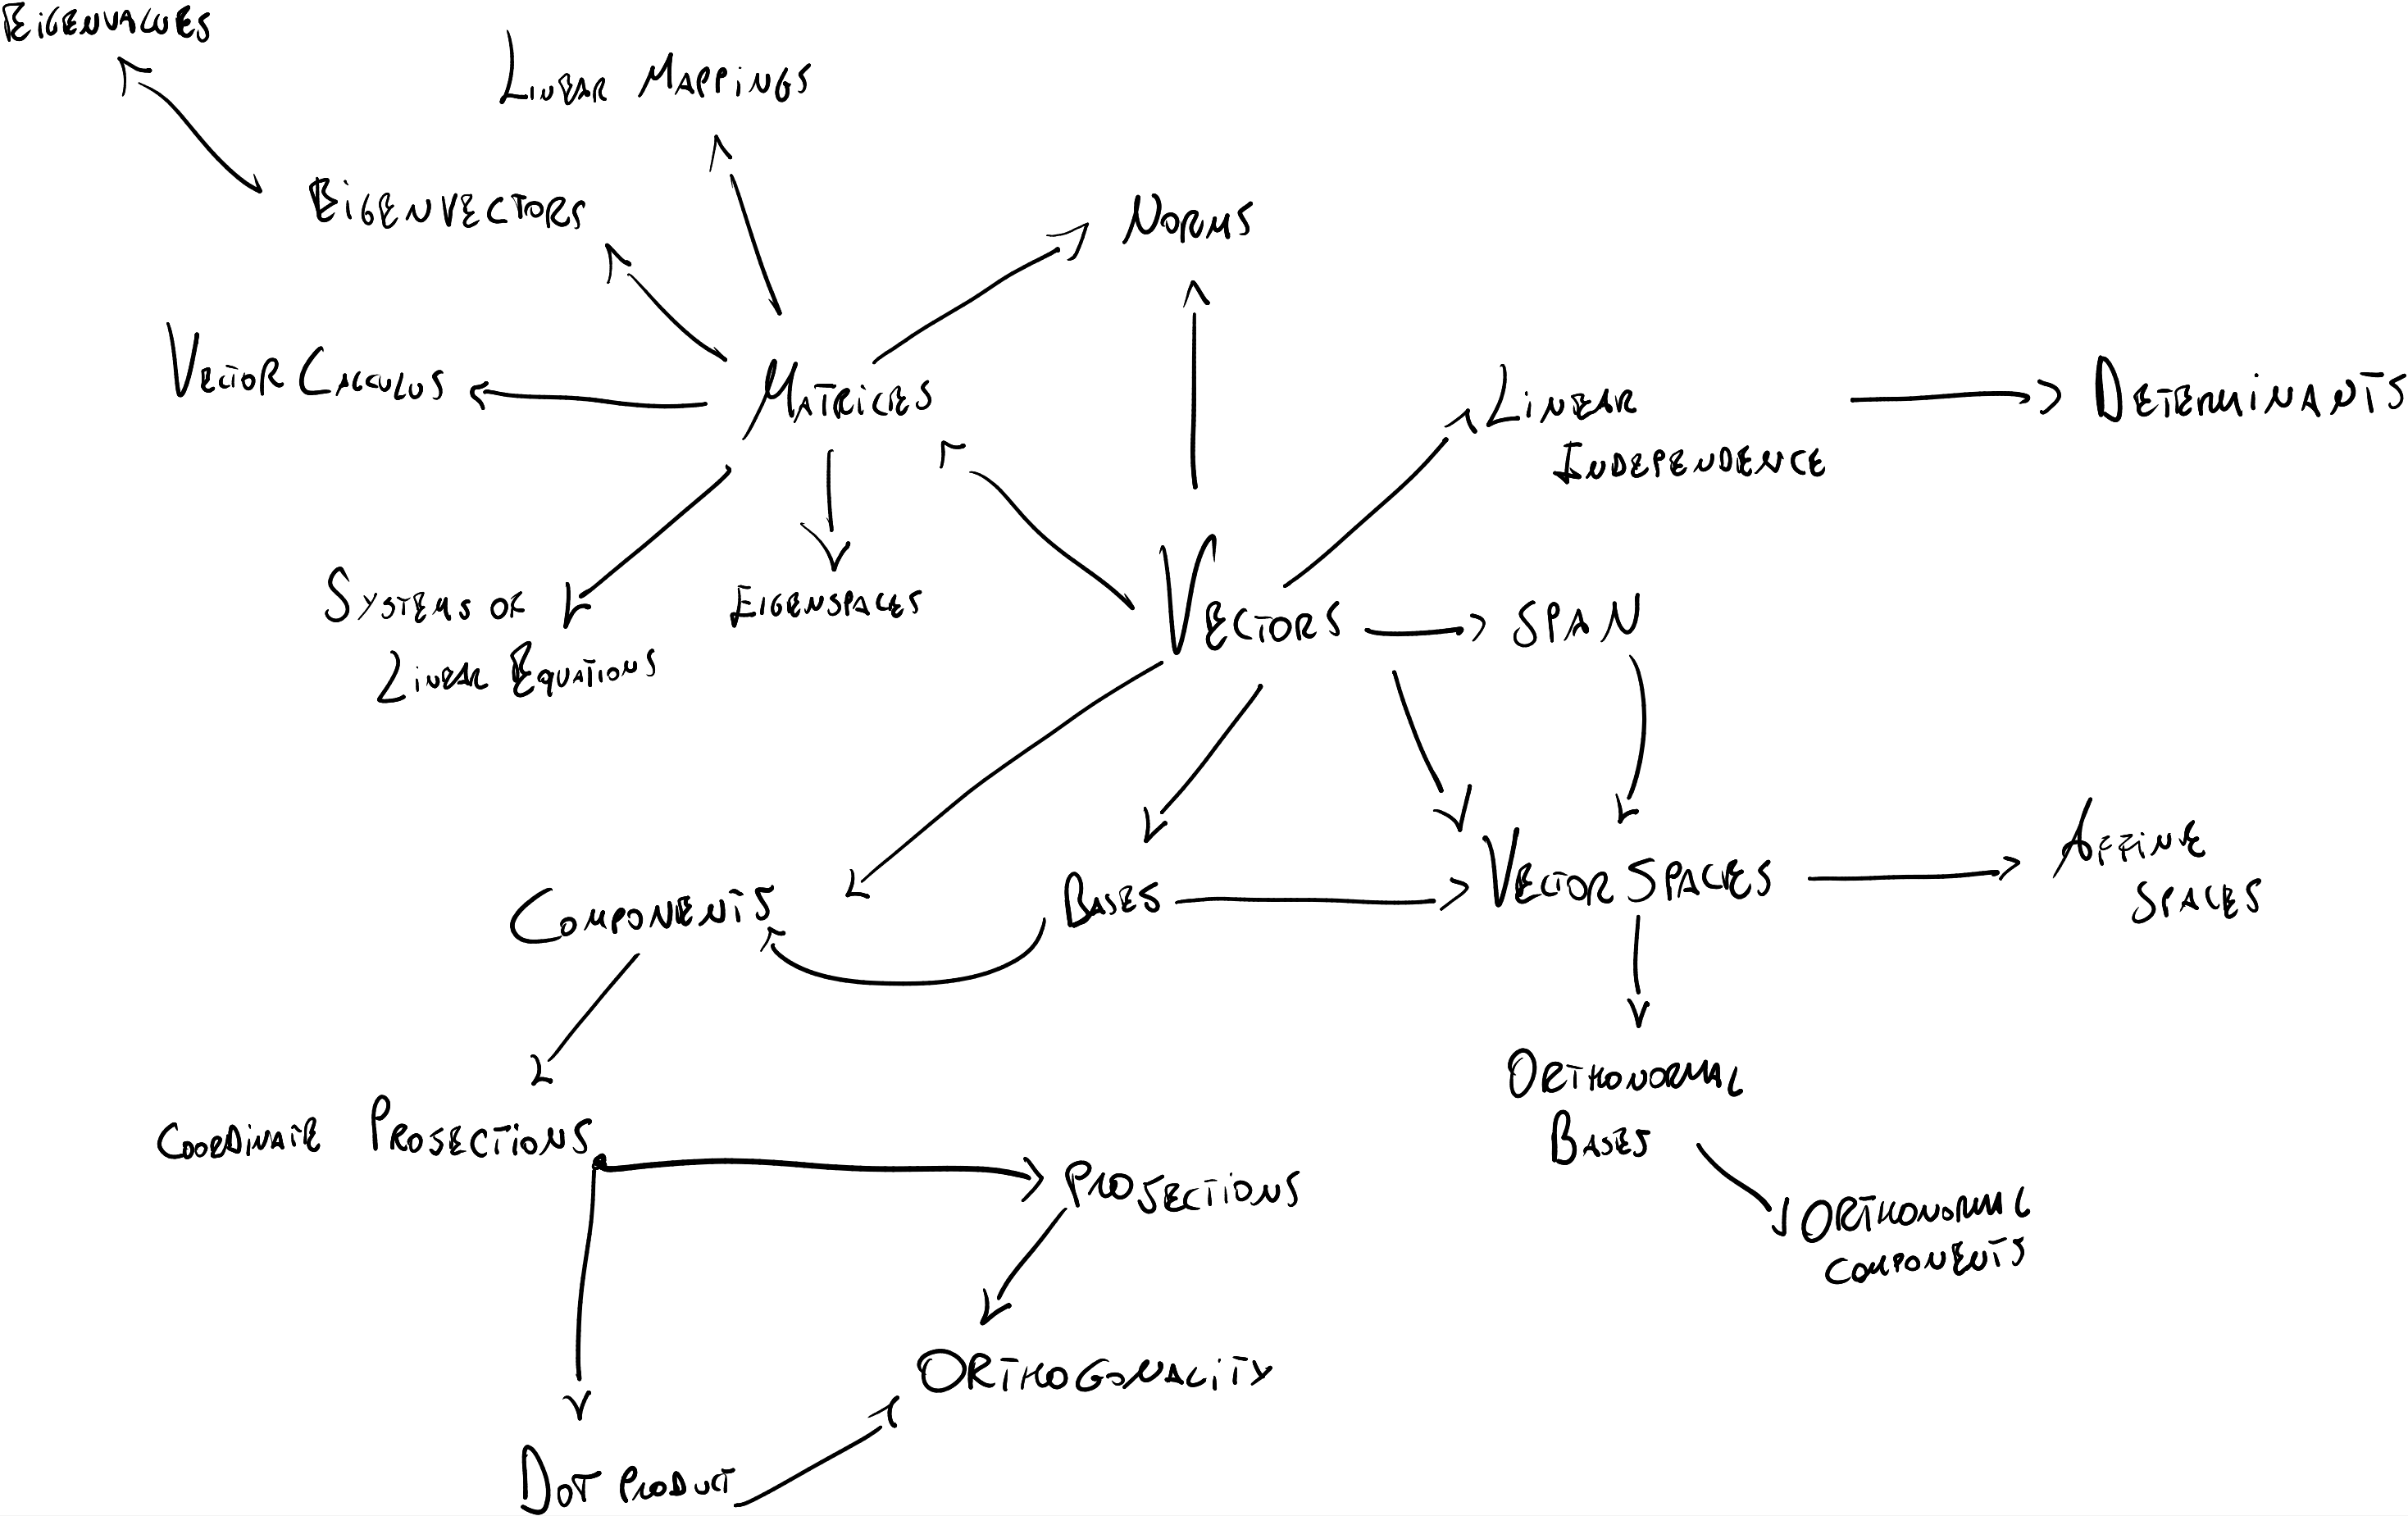
\includegraphics[scale=0.15]{Images/Linear_Algebra-map.png}
    \caption{Conceptual map of intersection of Linear Algebra and Analytic Geometry}
    \label{fig:conceptual-map}
\end{figure}

\noindent
Join me on this mathematical odyssey, where clarity, intuition, and computational prowess converge to make the abstract tangible. Let's unravel the beauty of linear algebra and analytic geometry, armed with the simplicity of Python programming, as we navigate through the pages of discovery and learning.

\section{Objects}
In the realm of mathematics, fundamental objects like scalars, vectors, matrices, and tensors serve as the building blocks for expressing a wide range of mathematical and scientific concepts. These entities encapsulate different levels of complexity, from singular values to multi-dimensional structures, each offering unique properties and applications.

\subsection{Scalars}
Scalars are elements of a field, like $\mathbb{R}$,that represent quantities that only have magnitude, such as temperature, mass, distance, or time. Scalars have zero dimensions. They are considered point values in a mathematical space.

Since a scalar has no dimensions, its shape is represented as an empty set.

Scalars are typically denoted by lowercase letters, e.g., $a,b,c$ and they are treated as constants; they can be real numbers, complex numbers, or elements from other mathematical fields.
\\

For example 

$$
a \in \mathbb{F}
$$

where is a scalar in a field $\mathbb{F}$.

\subsection{Vectors}
A vector is an ordered collection of elements of a field that represents a quantity with both magnitude and direction. Vectors are used to describe various physical quantities, such as displacement, velocity, and force.
In a geometric sense, they can be visualized as directed line segments with a specific length and direction in space.

Vectors have one dimension, so the shape of a vector is a 1-dimensional tuple $(n)$, where $n$ is the number of elements in the vector, also known as vector size. 
\\

Here are a few key points to understand about vectors:
\begin{itemize}
    \item \textbf{Magnitude:} This is the length of the vector.

    \item \textbf{Direction:} This indicates the way the vector points.

    \item \textbf{Components:} The individual parts that make up a vector.
\end{itemize}

They are typically denoted by a letter with an arrow above. For example

$$
\vec v =\begin{bmatrix}
    v_1\\
    v_2\\
    \vdots\\
    v_n
\end{bmatrix} \in \mathbb{F}^n,
$$

where $\vec v$ is a vector in $\mathbb F^n$, $(n)$ is the vector shape, $n$ is the vector size and $v_1, v_2, \dots, v_n \in \mathbb{F}$ are vector components.

If we wish to access the component within the vectors we can employ the following mathematical notation: 

$$
\vec v^{\ (1)} = v_1
$$

And to access all elements of a dimension we can use ":" instead of numerical indexes:

$$
\vec v^{\ (:)} = \vec v
$$

\subsection{Matrices}
A matrix is a two-dimensional array of elements of a field, organized in rows and columns. It is used to represent and manipulate data in various applications, including linear transformations and systems of equations.

The shape of a matrix is a 2-dimensional tuple $(m,n)$, where $m$ is the number of rows and $n$ is the number of columns. 

Matrices are typically denoted by uppercase letters, e.g., $A, B, C$. For example 

$$
A_{m,n} = \begin{bmatrix} 
    a_{11} & \dots  & a_{1n}\\
    \vdots & \ddots & \vdots\\
    a_{m1} & \dots  & a_{mn} 
\end{bmatrix} \in \mathbb{F}^{m \times n}
$$

where $A_{m,n}$ is a matrix in $\mathbb{F}^{m \times n}$, $(m, n)$ is the matrix shape and $a_{i,j} \in \mathbb F$.

If we wish to access the component within the matrix we can employ the following mathematical notation: 

$$
A_{m,n}^{(i, j)} = a_{i,j}
$$

And to access all elements of a dimension we can use ":" instead of numerical indexes:

$$
A_{m,n}^{(i, :)} = \begin{bmatrix}
    a_{i,1}\\
    a_{i, 2}\\
    \vdots\\
    a_{i, n}
\end{bmatrix}, \quad A_{m,n}^{(:, j)} = \begin{bmatrix}
    a_{1,j}\\
    a_{2,j}\\
    \vdots\\
    a_{m,j}
\end{bmatrix}, \quad  A_{m,n}^{(:, :)} = A_{m,n}
$$


\subsubsection{Square Matrices}

A square matrix $A_{m,n}$ is a matrix with the same number of rows and columns, i.e., $m = n$.

\subsubsection{Triangular Matrices}
A lower triangular matrix $A$ is a square matrix where all entries above the main diagonal are zero, i.e., $a_{i,j} = 0$ for $i < j$.

An upper triangular matrix $A$ is a square matrix where all entries below the main diagonal are zero, i.e., $a_{i,j} = 0$ for $i > j$.

\subsubsection{Diagonal Matrices}

A diagonal matrix $D$ is a square matrix where all entries outside the main diagonal are zero, i.e., $a_{i,j} = 0$ for $i \neq j$.

\subsubsection{Symmetric Matrices}
A symmetric matrix $A_{n,n}$ is a square matrix where the elements are symmetric with respect to the main diagonal. 
In other words, if $a_{i,j}$ is an entry in the matrix at the $i$-th row and $j$-th column, then $a_{i,j} = a_{j,i}$ 
for all $i$ and $j$ in the matrix. This symmetry implies that the values on one side of the main diagonal mirror the 
values on the other side.

% Diagonale di una matrice
%%Null matrix
\section{Basic Operations}
In the world of linear algebra, basic operations form the cornerstone of mathematical manipulations applied to our objects (scalar, vectors and matrices). These operations serve as fundamental tools for analyzing and transforming these mathematical entities, unlocking insights across various disciplines.

\subsection{Transposition}

In linear algebra, transposition refers to the operation of switching the rows and columns of a mathematical object. This operation is commonly applied to matrices, and geometrically can be interpreted as reflecting the matrix over its main diagonal.

\subsubsection{Matrices Transposition}

For a given matrix $A_{m,n} \in \mathbb F^{m \times n}$, the transpose, denoted as $A_{m,n}^T$, is obtained by swapping its rows with columns. Mathematically, each $a_{i,j}$ in $A_{m,n}$, would be mapped into $a_{ji}$. In other words, the element in the $i$-th row and $j$-th column of $A_{m,n}^T$ is the same as the element in the $j$-th row and $i$-th column of $A_{m,n}$.

So $A_{m,n}^T = A_{n,m}'$.
\\

\textbf{Example:}

Consider the following matrix:
\[
A = \begin{bmatrix}
    1 & 2 & 3 \\
    4 & 5 & 6 \\
    7 & 8 & 9 \\
\end{bmatrix}
\]

The transpose of matrix $A$ is:
\[
A^T = \begin{bmatrix}
    1 & 4 & 7 \\
    2 & 5 & 8 \\
    3 & 6 & 9 \\
\end{bmatrix}
\]

\subsubsection{Properties:}

\begin{itemize}
    \item $(A^T)^T = A$: Transposing a matrix twice results in the original matrix.
    \item $(cA)^T = cA^T$: Transposing a scaled matrix is equivalent to scaling the transpose.
    \item $(A + B)^T = A^T + B^T$: Transposing the sum of two matrices is equivalent to the sum of their transposes.
\end{itemize}

These properties are fundamental in various mathematical applications, including linear algebra and optimization.


\subsection{Addition}
In linear algebra, the sum of two objects is a fundamental operation that combines their respective components.
We are very familiar with the common sum of scalars:

$$
a + b = c,
$$
but what happens when we need to apply the sum to objects of dimension greater than 0?
\\

Vector sum, for example is defined as follow. 
\\

Let 
$$
\vec{v} = \begin{bmatrix} v_1 \\ v_2 \\ \vdots \\ v_n \end{bmatrix}, \quad \vec{w} = \begin{bmatrix} w_1 \\ w_2 \\ \vdots \\ w_n \end{bmatrix}
$$
be two vectors in \(\mathbb{F}^n\). 
    The sum of two vectors \(\vec{v}\) and \(\vec{w}\), denoted as \(\vec{v} + \vec{w}\), is defined component-wise:
    
\[ \vec{v} + \vec{w} = \begin{bmatrix} v_1 + w_1 \\ v_2 + w_2 \\ \vdots \\ v_n + w_n \end{bmatrix} \]

Geometrically, vector addition corresponds to placing the initial point of the second vector at the terminal point of the first vector and connecting the initial point of the first vector to the terminal point of the second vector (as shown in Figure \ref{fig:vector-sum-1}).
\\
\begin{figure}[h]
    \centering
    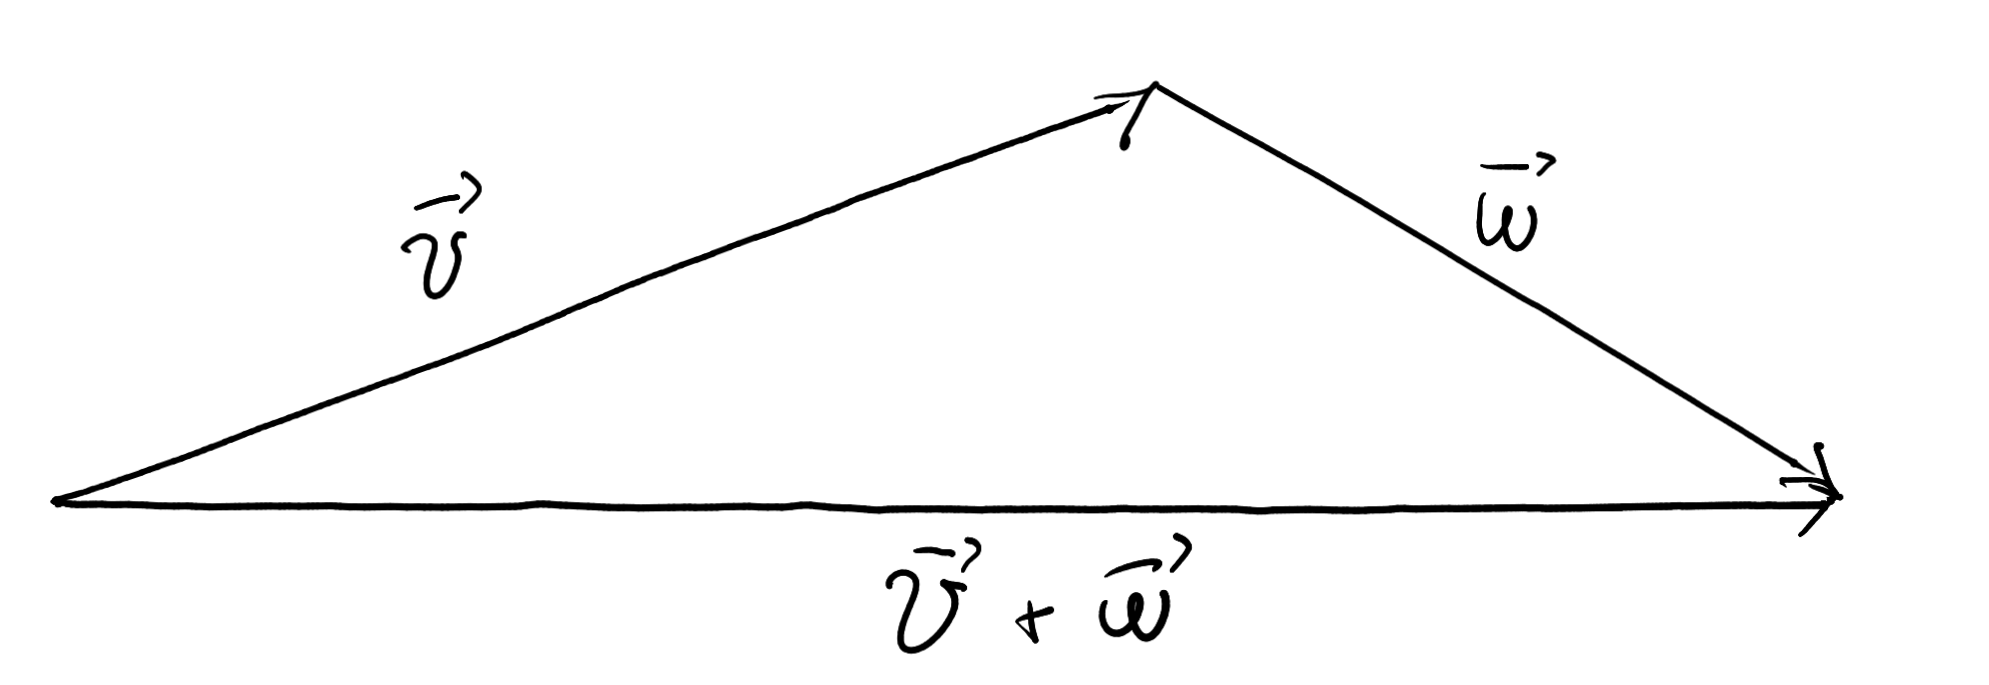
\includegraphics[scale=0.2]{Images/Linear_Algebra-vector-sum1.png}
    \caption{Triangle Law of Vector Addition}
    \label{fig:vector-sum-1}
\end{figure}

Now, let's consider an example of vector addition using two real vectors, $\vec a$ and $\vec b$. The sum of $\vec a$ and $\vec b$ will be:

$$
\vec a = \begin{bmatrix}
    1 \\
    2
\end{bmatrix}
\quad
\vec b = \begin{bmatrix}
    2 \\
    -3
\end{bmatrix}
$$

$$
\vec a + \vec b = \begin{bmatrix}
    a_0 + b_0 \\
    a_1 + b_1
\end{bmatrix} = \begin{bmatrix}
    1 + 2 \\
    2 + (-3)
\end{bmatrix} = \begin{bmatrix}
    3 \\
    -1
\end{bmatrix}
$$

\begin{figure}[h]
    \centering
    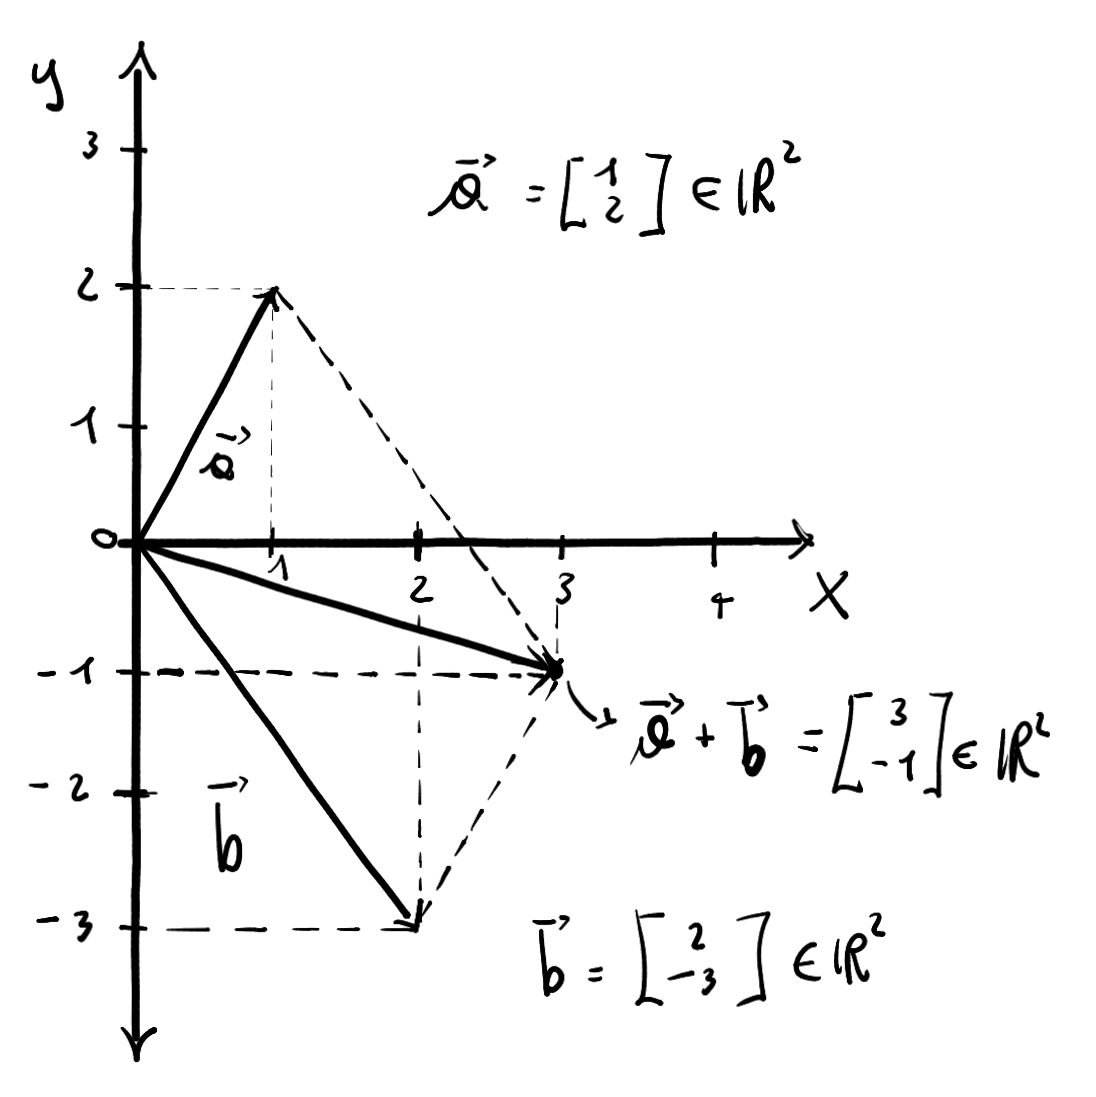
\includegraphics[scale=0.25]{Images/Linear_Algebra-vector-sum2.png}
    \caption{Parallelogram Law of Addition of Vectors}
    \label{fig:vector-sum-2}
\end{figure} 

The Figure \ref{fig:vector-sum-2} shows the vector sum graphically by using the Parallelogram law.

Note that we can sum together only vectors that have the same shape.
\\

The same concept can be applied to matrices, in fact given two matrices 

$$
A_{m,n} = \begin{bmatrix}
    a_{1,1} & a_{1,2} & \dots & a_{1,n} \\
    a_{2,1} & a_{2,2} & \dots & a_{2,n} \\
    \vdots & \vdots & \ddots & \vdots \\
    a_{m,1} & a_{m,2} & \dots & a_{m,n}
\end{bmatrix}, \quad
B_{m,n} = \begin{bmatrix}
    b_{1,1} & b_{1,2} & \dots & b_{1,n} \\
    b_{2,1} & b_{2,2} & \dots & b_{2,n} \\
    \vdots & \vdots & \ddots & \vdots \\
    b_{m,1} & b_{m,2} & \dots & b_{m,n}
\end{bmatrix}
$$

their sum is defined as

\[
A_{m,n} + B_{m,n} =
\begin{bmatrix}
    a_{1,1} + b_{1,1} & \dots & a_{1,n} + b_{1,n} \\
    a_{2,1} + b_{2,1} & \dots & a_{2,n} + b_{2,n} \\
    \vdots & \ddots & \vdots \\
    a_{m,1} + b_{m,1} & \dots & a_{m,n} + b_{m,n}
\end{bmatrix}
=
\begin{bmatrix}
    c_{1,1} & \dots & c_{1,n} \\
    c_{2,1} & \dots & c_{2,n} \\
    \vdots & \ddots & \vdots \\
    c_{m,1} & \dots & c_{m,n}
\end{bmatrix}
= C_{m,n}
\]

or, more mathematically, the generic $c_{i,j}$ of $C_{m,n}$ of new matrices is equal to $a_{i,j} + b_{i,j}$.
Note that we can sum together only matrices that have the same shape.
\\

\subsection{Sum Over Axes}\label{subsection:sum-over-axes}
Now, let's introduce the concept of \textit{sum over axes}.

The \textit{sum over axes} operation plays a crucial role, particularly when dealing with high dimensionality objects. This operation allows us to efficiently contract algebraic objects along specified axes, resulting in a new object with reduced dimension.

Consider a very simple example, imagining having a vector $\vec{v} \in \mathbb{F}^n$ and wanting to perform a \textit{sum over axes} on its (only) axis, i.e., axis 0.

$$
\vec{v} = \begin{bmatrix}
    v_1 \\
    v_2 \\
    \vdots\\
    v_n
\end{bmatrix} \in \mathbb{F}^n \quad \underset{\text{Sum over 0 axis}}{\longrightarrow} = \sum_{i=0}^n v_i
$$

After the sum over the 0 axis of the vector $\vec{v}$, we obtain a scalar belonging to the same field as the vector components. 
\\

So, for example:

\[
\vec{v} = \begin{bmatrix}
    1 \\
    2 \\
    3
\end{bmatrix} \in \mathbb{F}^3 \quad \underset{\text{Sum over 0 axis}}{\longrightarrow} 
\begin{bmatrix}
    1 + 2 + 3
\end{bmatrix} = 6 \in \mathbb{F}
\]

Consider another very simple example, imagining having a matrix $A_{m,n}$ and wanting to perform a \textit{sum over axes} on axis 0.

$$
A_{m,n} = \begin{bmatrix}
    a_{1,1} & a_{1,2} & \dots & a_{1,n} \\
    a_{2,1} & a_{2,2} & \dots & a_{2,n} \\
    \vdots & \vdots & \ddots & \vdots \\
    a_{m,1} & a_{m,2} & \dots & a_{m,n}
\end{bmatrix}  \in \mathbb{F}^{m \times n} \quad \underset{\text{Sum over 0 axis}}{\longrightarrow} A_{1, n}' = 
\begin{bmatrix}
    \sum_{i=0}^m a_{i,1} & \sum_{i=0}^m a_{i,2} & \dots & \sum_{i=0}^m a_{i,n}
\end{bmatrix}
$$

For example:

\[
A_{3,4} = \begin{bmatrix}
    1 & 2 & 3 & -8 \\
    2 & 5 & -1 & 9 \\
    3 & 3 & -7 & -2
\end{bmatrix} \in \mathbb{F}^{3 \times 4} \quad \underset{\text{Sum over 0 axis}}{\longrightarrow} A_{1, 4}' = 
\begin{bmatrix}
    1 & 2 & 3 & -8 \\
    + & + & + & + \\
    2 & 5 & -1 & 9 \\
    + & + & + & + \\
    3 & 3 & -7 & -2
\end{bmatrix}
=
\begin{bmatrix}
    6 & 10 & -5 & -1
\end{bmatrix}
\]

Thus, we have obtained the \textit{sum over axes} on axis 0 of the matrix $A_{5,4}$, obtaining a row vector $A'$ of one dimension and size 4.

Similarly, if we wanted to perform a \textit{sum over axes} on axis 1, we would get

$$
A_{mn} = \begin{bmatrix}
    a_{1,1} & a_{1,2} & \dots & a_{1,n} \\
    a_{2,1} & a_{2,2} & \dots & a_{2,n} \\
    \vdots & \vdots & \ddots & \vdots \\
    a_{m,1} & a_{m,2} & \dots & a_{m,n}
\end{bmatrix} \in \mathbb{F}^{m \times n} \quad \underset{\text{Sum over 1 axis}}{\longrightarrow} A_{m, 1}' =
\begin{bmatrix}
    \sum_{i=0}^n a_{1,i} \\
    \sum_{i=0}^n a_{2,i} \\
    \vdots\\
    \sum_{i=0}^n a_{m,i}
\end{bmatrix}
$$
For example:
\[
A_{3,4} = \begin{bmatrix}
    1 & 2 & 3 & -8 \\
    2 & 5 & -1 & 9 \\
    3 & 3 & -7 & -2
\end{bmatrix} \in \mathbb{F}^{3 \times 4} \quad \underset{\text{Sum over 1 axis}}{\longrightarrow} A_{3, 1}' = 
\begin{bmatrix}
    1 + 2 + 3 - 8 \\
    2 + 5 - 1 + 9 \\
    3 + 3 - 7 - 2
\end{bmatrix}
=
\begin{bmatrix}
    -2 \\
    15 \\
    -3
\end{bmatrix}
\]


\subsection{Multiplication}
When we talk about product, we are, of course, referring to the multiplication between two algebraic objects. When these two objects are scalars, we don't need to consider the issue of dimensionality, as scalars are objects with no dimension, and therefore, their product will inevitably have no dimension. However, as the complexity (and hence, dimension) of the objects we want to multiply increases and differs between the two objects, we need to take into account not only the product itself, but also the dimensional differences involved. In fact, as the shape of the objects increases (and differs), the possible ways of performing their product also increase.

In the following sections, it will become clearer in what ways it is possible to perform the standard product between two objects (scalar, vectors or matrices) and what is the difference with standard product, \textbf{Hadamard} product and \textbf{Kronecker} product.

Esistono molti modi di calcolare il prodotto tra due ogetti algebrici, ma la caratteristica che li accomuna è che tutti i prodotti si basano su due operazioni fondamentali:

\begin{itemize}
    \item Sum over axes.
    \item Moltiplicazione tra scalari.
\end{itemize}

Dove la \textit{sum over axes}, precedentemente introdotta nella sottosezione \ref{subsection:sum-over-axes}, ci permette di eseguire le operazioni di contrazione degli assi necessarie al calcolo del prodotto di due ogetti algebrici.

Mentre il prodotto standard tra scalari è il normale prodotto a cui siamo abituati; definito per due generici elementi $a, b$ del campo $\mathbb{F}$ come:

$$
a \cdot b = c \in \mathbb{F}
$$

Tramite queste due operazioni siamo in grado di eseguire il prodotto di due elementi algebrici di dimensionalità arbitraria.

\subsubsection{Compatibilità tra Assi}

Prima di addentrarci nel calcolo vero e proprio, dobbiamo chiarire anche un altro punto, senza il quale non è possibile eseguire tutte le tipologie di prodotto. Introduciamo quindi il concetto di \textit{compatibilità tra assi}: due assi (dimensioni) si dicono compatibili se e solo se hanno la stessa size (contengono lo stesso numero di elementi). Per asse si intende la dimensione, ad esempio l'asse 0 (l'unico) del vettore $\vec v \in  \mathbb{F}^n$ è la sua dimensione, l'asse del vettore $\vec w \in \mathbb{F}^m$ sono compatibili se e solo se $n = m$. 

Facciamo un altro esempio, siano $A_{3, 2} \in \mathbb{F}^{3 \times 2}$ e $B_{2, 3} \in \mathbb{F}^{2 \times 3}$ due matrici, in questo caso l'asse 0 della matrice $A_{3,2}$ e l'asse 1 della matrice $B_{2, 3}$ sono compatibili, ma anche l'asse 1 della matrice $A_{3,2}$ e l'asse 0 della matrice $B_{2,3}$ lo sono.

Mentre eseguiamo il prodotto di due ogetti algebrici, può essere necessario tenere conto di quali assi sono compatibili, perchè alcuni tipi di prodotto necessitano tale requisito.

\subsubsection{Prodotto}
In generale il prodotto tra due generici ogetti algebrici viene calcolato attraverso una prima fase di scelta degli assi compatibili sui quali effettuare la contrazione, e una seconda fase nella quale si effettua il broadcast sulle dimensioni che non sono state scelte per la contrazione. In generale il risultato è dato da un ogetto che ha per dimensioni tutte le dimensioni "non scelte" in ordine di moltiplicazione. 

In questa sezione ci limiteremo a descrivere le principali metodologie di calcolo del prodotto.
\\
 
L'esempio più semplice (escluso il prodotto tra scalari) è il prodotto di uno scalare per un vettore. In questo caso non si scelgono assi compatibili (perché non ve ne sono) quindi non si effettua la contrazione, ma si passa direttamente alla fase di broadcast dello scalare per ogni componente del vettore. Tale prodotto è definito tra uno scalare $a \in \mathbb F$ e un vettore $\vec v \in \mathbb{F}^n$ e si scrive

$$
a \cdot \vec v = a \cdot \begin{bmatrix}
    v_1\\
    v_2\\
    \vdots\\
    v_n
\end{bmatrix} = \begin{bmatrix}
    a \cdot v_1\\
    a \cdot v_2\\
    \vdots\\
    a \cdot v_n
\end{bmatrix} \in \mathbb F^{n}.
$$

Il risultato è un vettore con la stessa size del vettore moltiplicato. Infatti se prendiamo la shape dello scalare $()$ e la shape del vettore $(n)$ e le mettiamo insieme otteniamo la shape del vettore risultato, che, dato che lo scalare non ha dimensioni, è proprio $(n)$.
\\
\iffalse
Facciamo però un esempio concreto: siano $\vec v = \beg$
\begin{figure}[h]
    \centering
    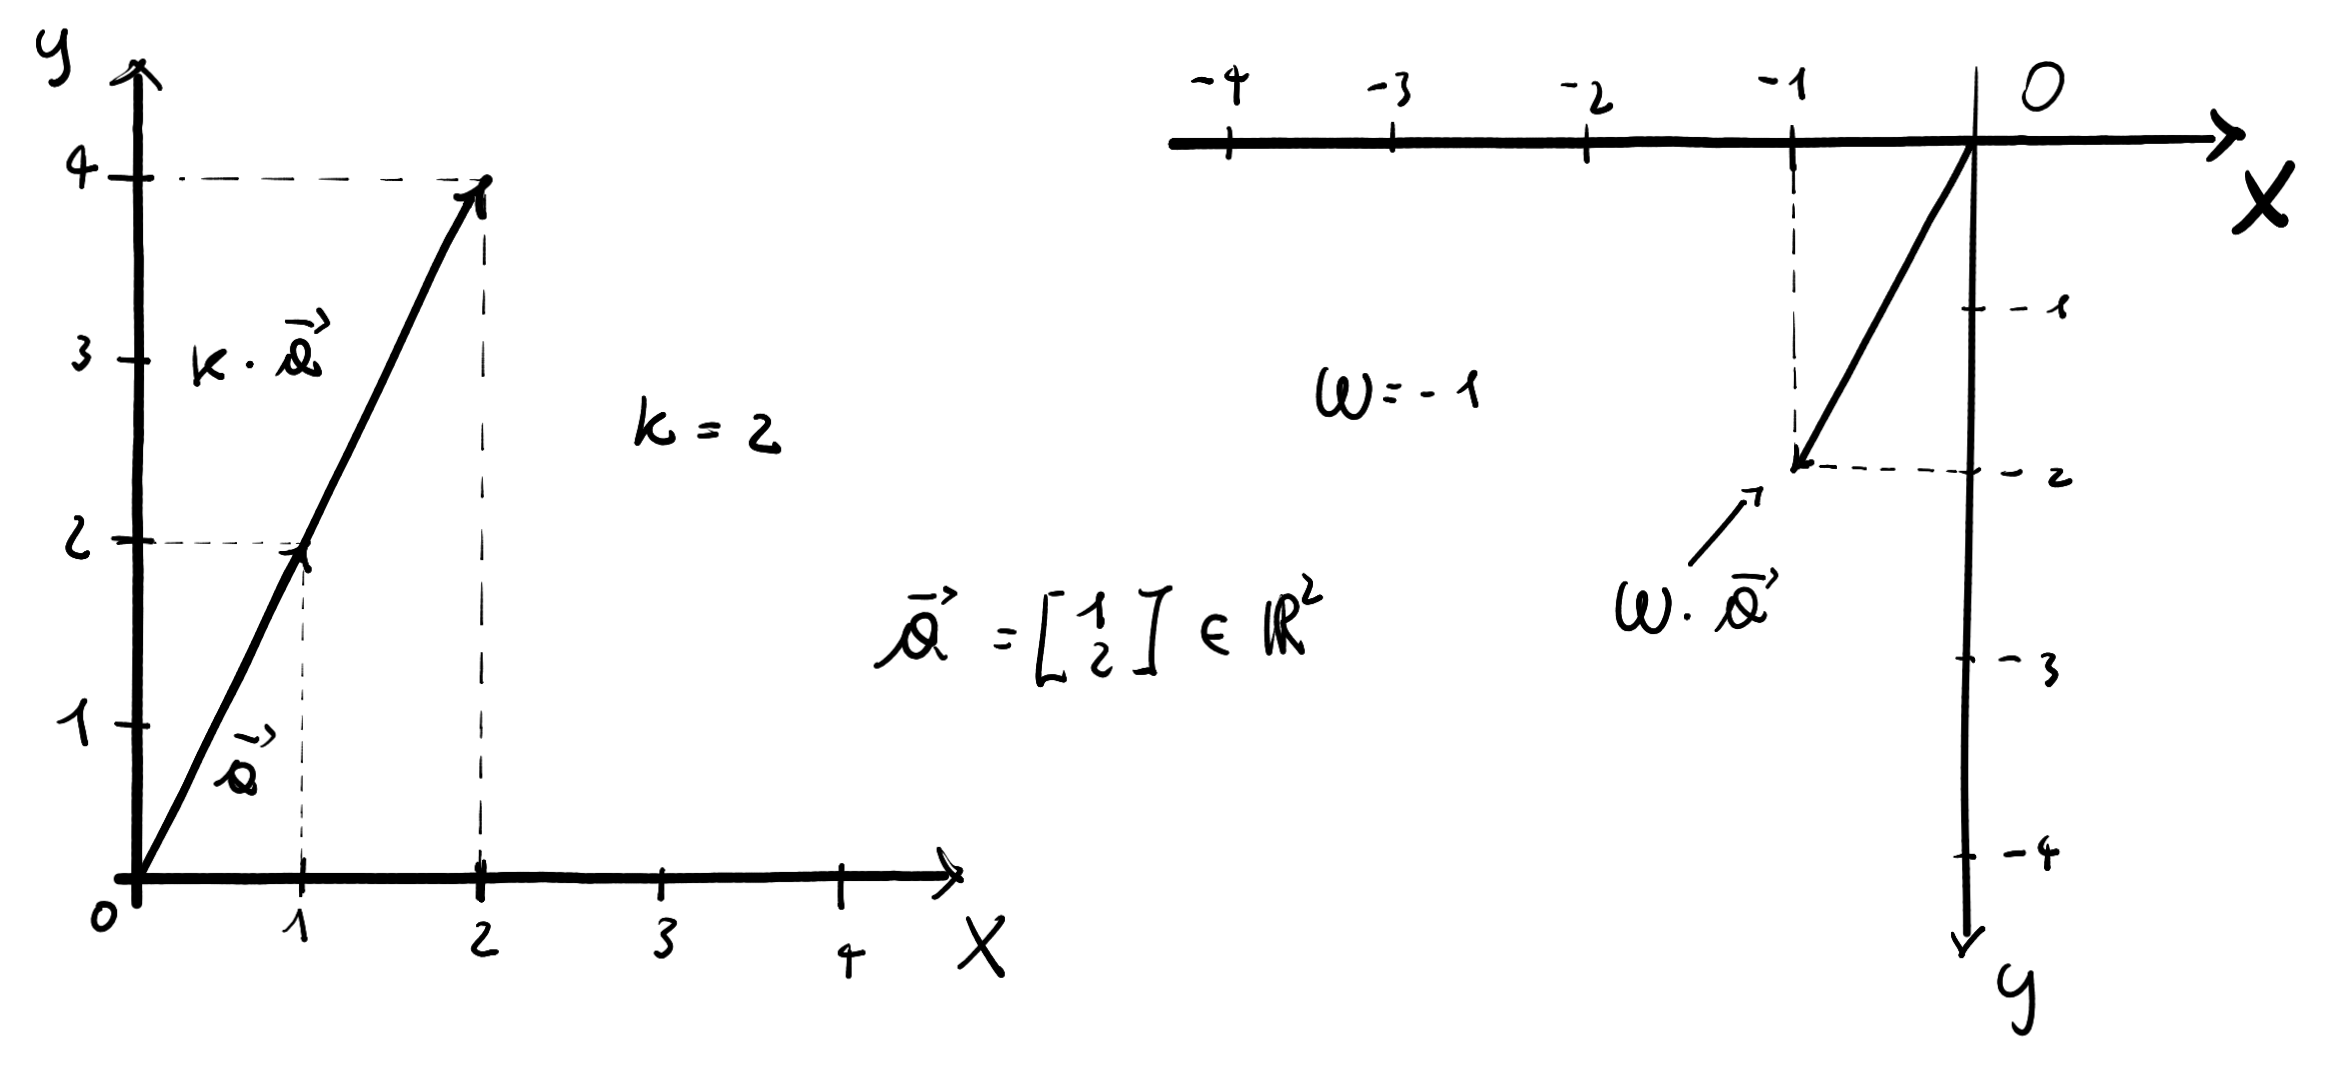
\includegraphics[scale=0.18]{Images/Linear_Algebra-scalar-mul.png}
    \caption{}
    \label{fig:scalar-mul}
\end{figure} 
\fi

Allo stesso modo, il prodotto tra uno scalare $a \in \mathbb F$ e una matrice $B_{m,n} \in\mathbb F^{m \times n}$ è definito come 

$$
a \cdot B_{m,n} = a \cdot \begin{bmatrix}
    b_{1,1} & \dots & b_{1,n}\\
    b_{2,1} & \dots & b_{1,n}\\
    \vdots  & \ddots & \vdots \\
    b_{m,1} & \dots & b_{m,n}
\end{bmatrix} = \begin{bmatrix}
    a \cdot b_{1,1} & \dots & a \cdot b_{1,n}\\
    a \cdot b_{2,1} & \dots & a \cdot b_{1,n}\\
    \vdots  & \ddots & \vdots \\
    a \cdot b_{m,1} & \dots & a \cdot b_{m,n}
\end{bmatrix} \in \mathbb F^{m \times n}.
$$

Da notare che, come nel caso precedente, lo scalare e la matrice non hanno dimensioni (assi) compatibili, quindi lo scalare viene moltiplicato per tutti i valori della matrice (broadcast). Come risultato finale abbiamo un ogetto che ha per dimensioni le dimensioni dello scalare, che non ne ha, e le dimenisoni della matrice, e quindi $(m,n)$.
\\

Un altro importante prodotto è il prodotto tra vettori. Il \textbf{Dot Product} tra vettori è definito come segue: dati due vettori $\vec v \in  \mathbb{F}^n$ e $\vec w \in \mathbb{F}^n$, il loro prodotto è definito come:

$$
\vec v \cdot \vec w = \begin{bmatrix}
        v_1\\
        \vdots \\
        v_n \\
\end{bmatrix}
    \cdot 
\begin{bmatrix}
        w_1\\
        \vdots \\
        w_n\\
\end{bmatrix} = \sum_{i=0}^n v_i \cdot w_i
$$

Come possimao osservare, scegliendo come assi compatibili: l'asse 0 del primo vettore e l'asse 0 del secondo; possiamo calcolare il prodotto element-wise delle componenti dei due vettori e successivamente, tramite la sum over axes, effettuiamo una contrazione sugli assi compatibili. Come notiamo, non ci sono dimensioni oltre a quelle che abbiamo selezionato, quindi il risultato avrà zero dimensioni e dunque sarà uno scalare.
\\

\`E possibile anche la moltiplicazione tra una matrice ed un vettore. Siano $A_{m,n} \in \mathbb F^{m \times n}$ una matrice e $\vec v \in \mathbb{F}^n$ un vettore. Il loro prodotto è definito come segue:

$$
A_{m,n} \cdot \vec v = \cdot \begin{bmatrix}
    a_{1,1} & \dots & a_{1,n}\\
    a_{2,1} & \dots & a_{1,n}\\
    \vdots  & \ddots & \vdots \\
    a_{m,1} & \dots & a_{m,n}
\end{bmatrix} \cdot \begin{bmatrix}
        v_1\\
        v_2\\
        \vdots \\
        v_n \\
\end{bmatrix} = \begin{bmatrix}
        \sum_{i=0}^n a_{1,i} \cdot v_i\\
        \sum_{i=0}^n a_{2,i} \cdot v_i\\
        \vdots \\
        \sum_{i=0}^n a_{n,i} \cdot v_i \\
\end{bmatrix} \in \mathbb F^{m}
$$

Notiamo che come assi compatibili abbiamo scelto l'unico asse (0) del vettore $\vec v$ e l'asse 1 della matrice $A_{m,n}$, e quindi la contrazione avviene su questa coppia di assi.
Il risultato, come vediamo, ha per dimensioni gli assi non scelti come compatibili nel prodotto, quindi solo l'asse 0 della matrice, che ha come size $m$.

Vediamo ora un esempio con due matrici: siano $A_{m,n} \in \mathbb{F}^{m \times n}$ e $B_{r,s} \in \mathbb{F}^{r \times s}$ due matrici con un asse compatibile (quindi ad esempio $n=r$), il loro prodotto è definito come

$$
A_{m,n} \cdot B_{r,s} = \begin{bmatrix}
    \sum_{i=0}^n a_{1,i} \cdot b_{i,1} & \dots & \sum_{i=0}^n a_{1,i} \cdot b_{i,s}\\
    \vdots & \ddots & \vdots\\
    \sum_{i=0}^n a_{m,i} \cdot b_{i,1} & \dots & \sum_{i=0}^n a_{m,i} \cdot b_{i,s}
\end{bmatrix} = C_{m,s}.
$$

Abbiamo ottenuto una matrice $C_{m,s}$ che ha lo stesso numero di righe di $A_{m,n}$ e lo stesso numero di colonne di $B_{r, s}$.

Questo è il prodotto matriciale standard più comunemente utilizzato; ve ne sono molti altri che si ottengono facendo una scelta diversa degli assi compatibili su cui fare la contrazione.
\\

C'è poi un altro particolare prodotto element-wise, che si effettua sugli assi compatibili, ma senza alcuna contrazione. Questo tipo di prodotto si chiama \textbf{Hadamard product} ed è definito solamente per ogetti algebrici con la stessa shape (stesso numero di assi e stassa size per ogni asse).

L'\textbf{Hadamard product} per la generica coppia di vettori $\vec v, \vec w \in \mathbb F^n$ è definito come

$$
\vec v \odot \vec w = \begin{bmatrix}
        v_1\\
        v_2\\
        \vdots \\
        v_n \\
\end{bmatrix} \odot \begin{bmatrix}
        w_1\\
        w_2\\
        \vdots \\
        w_n \\
\end{bmatrix} = \begin{bmatrix}
        v_1 \cdot w_1\\
        v_2 \cdot w_2\\
        \vdots \\
        v_n \cdot w_n\\
\end{bmatrix} \in \mathbb F^{n}.
$$

Analogamente nel caso di due matrici $A_{m,n}, B_{m,n}$ il loro \textbf{Hadamard product} è definito come 

$$
A_{m,n} \odot B_{m,n} = \begin{bmatrix}
    a_{1,1} \cdot b_{1,1} & \dots & a_{1,n} \cdot b_{1,n}\\
    \vdots & \ddots & \vdots\\
    a_{m,1} \cdot b_{m,1} & \dots & a_{m,n} \cdot b_{m,n}
\end{bmatrix} \in \mathbb F^{m \times n}.
$$

In questa sezione sono state illustrate solamente alcune delle tipologie di prodotto che è possibile effettuare nell'algebra lineare. Questo perché si tratta di un testo introduttivo, dove vengono trattati solamente gli aspetti basici dell'algebra lineare che è una materia molto profonda.
\section{Gaussian Elimination}
Gaussian elimination, also known as row reduction, is an algorithm primarily used for solving systems of linear equations. It involves a series of row-wise operations performed on the corresponding matrix of coefficients. This method can be extended to compute the rank of a matrix, the determinant of a square matrix, and the inverse of an invertible matrix. Named after Carl Friedrich Gauss (1777–1855), it serves as a fundamental technique in linear algebra.

To perform row reduction on a matrix, one applies a sequence of elementary row operations to transform the matrix until the lower left-hand corner is filled with zeros, as much as possible. There are three types of elementary row operations:

\begin{enumerate}
    \item Swapping two rows,
    \item Multiplying a row by a nonzero number,
    \item Adding a multiple of one row to another row.
\end{enumerate}

Using these operations, a matrix can always be transformed into an upper triangular matrix, and indeed one that is in \textit{row-echelon form} (\textbf{REF}).

%Teorema sull'equivalenza dopo le operazioni di riga

%%%%%%%%%%%%%%%%%%%%%%%%%       DIM      %%%%%%%%%%%%%%%%%%%%%%%%%%%%%%%%%%%%



%%%%%%%%%%%%%%%%%%%%%%%%%%%%%%%%%%%%%%%%%%%%%%%%%%%%%%%%%%%%%%%%%%%%%%%%%%%%%

\subsection{Gauss-Jordan Algorithm}

The Gauss-Jordan algorithm is an extension of the Gaussian elimination method, aiming to transform matrix into \textit{reduced row-echelon form} (\textbf{RREF}).
\\
First of all we have to give the definition of \textit{row operation} and explain what the \textbf{RREF} is.
\\

\textbf{Reduced Row-echelon Form}

Reduced row-echelon form is a specific form that a matrix can be transformed into through row operations. A matrix is in reduced row-echelon form if it satisfies the following conditions:

\begin{enumerate}
    \item In each row, the left-most nonzero entry is 1 and the column that contains this 1 has all other entries equal to 0. This 1 is called a leading 1.

    \item The leading 1 in the second row or beyond is to the right of the leading 1 in the row just above.

    \item Any row containing only 0s is at the bottom.
\end{enumerate}

For example

\[
\begin{bmatrix}
0 \cdots 0 & 1_{1,j_1} \ 0 & \cdots & \cdots & \cdots & \cdots & \cdots & \cdots & 0\\
0 \cdots 0 & \cdots  & 0 & 1_{2,j_2} \ 0 & \cdots & \cdots & \cdots & \cdots & 0\\
\vdots&&\vdots&&\vdots&&\vdots\\
0 \cdots 0 & \cdots & 0 & \cdots & 0 & \cdots & 1_{r,j_r} \ 0& \cdots & 0\\
\vdots&&\vdots&&\vdots&&\vdots\\
0 \cdots 0 &\cdots & \cdots & \cdots & \cdots & \cdots & \cdots & \cdots & 0\\
\end{bmatrix}
\]

Where the first nonzero element of each row is equal to $1$ and has $j_k \geq i$; and all $a_{r,j_k}$ with $r \neq i$ are equal to zero.
\\

\section{Inverse of a Matrix}

The Gauss-Jordan elimination method is a systematic way to find the inverse of a matrix by transforming it into reduced row-echelon form. Let's denote the given matrix as $A$:

\[
A = \begin{bmatrix}
    a & b \\
    c & d
\end{bmatrix}
\]

To find the inverse of $A$ using Gauss-Jordan elimination, we will form an augmented matrix by appending the identity matrix of the same size next to $A$. Then, we will perform row operations until $A$ becomes the identity matrix, and the inverse of $A$ will be on the other side of the augmented matrix.

\textbf{Example:} Let's find the inverse of the matrix $A = \begin{bmatrix} 2 & 3 \\ 1 & 2 \end{bmatrix}$ using Gauss-Jordan elimination.

We start with the augmented matrix:

\[
\begin{bmatrix}
    2 & 3 & | & 1 & 0 \\
    1 & 2 & | & 0 & 1
\end{bmatrix}
\]

We perform row operations to transform the left side of the matrix into the identity matrix:

1. Subtract $\frac{1}{2}$ times the first row from the second row:

\[
\begin{bmatrix}
    2 & 3 & | & 1 & 0 \\
    0 & 1 & | & -\frac{1}{2} & 1
\end{bmatrix}
\]

2. Subtract $3$ times the second row from the first row:

\[
\begin{bmatrix}
    2 & 0 & | & \frac{7}{2} & -3 \\
    0 & 1 & | & -\frac{1}{2} & 1
\end{bmatrix}
\]

3. Divide the first row by $2$:

\[
\begin{bmatrix}
    1 & 0 & | & \frac{7}{4} & -\frac{3}{2} \\
    0 & 1 & | & -\frac{1}{2} & 1
\end{bmatrix}
\]

Therefore, the inverse of matrix $A$ is $\begin{bmatrix} \frac{7}{4} & -\frac{3}{2} \\ -\frac{1}{2} & 1 \end{bmatrix}$.

\chapter{Vector spaces}
\section{Introduction}

A vector space over a field \(\mathbb F\) is a non-empty set \(V\) together with two binary operations. It is indicated as a triplet: $(V, +, \cdot)$.

A vector space must satisfy the ten axioms listed below.

{\large$$\forall \vec v, \vec w, \vec u \in V \land \forall a, b \in \mathbb F$$}

\begin{itemize}
\item \textbf{Closure under "+" operation:}
    $\vec v + \vec w \in V$
\item \textbf{Closure under "·" operation:}
    $a \cdot \vec v \in V$
\item \textbf{Associativity of vector addition:} $\vec{u} + (\vec{v} + \vec{w}) = (\vec{u} + \vec{v}) + \vec{w}$
\item \textbf{Commutativity of vector addition:} $\vec{u} + \vec{v} = \vec{v} + \vec{u}$
\item \textbf{Identity element of vector addition:} There exists an element $\vec{0} \in V$, called the zero vector, such that $\vec{v} + \vec{0} = \vec{v}$.
\item \textbf{Inverse elements of vector addition:} $\exists -\vec{v} \in V$ called the additive inverse of $\vec{v}$, such that $\vec{v} + (-\vec{v}) = \vec{0} \in V$.
\item \textbf{Compatibility of scalar multiplication with field multiplication:} $a(b\vec{v}) = (ab)\vec{v}$.
\item \textbf{Identity element of scalar multiplication:} $1\vec{v} = \vec{v}$ where $1$ denotes the multiplicative identity in $\mathbb F$.
\item \textbf{Distributivity of scalar multiplication with respect to vector addition:} $a(\vec{u} + \vec{v}) = a\vec{u} + a\vec{v}$.
\item \textbf{Distributivity of scalar multiplication with respect to field addition:} $(a + b)\vec{v} = a\vec{v} + b\vec{v}$.
\end{itemize}

In this context, the elements of \(V\) are commonly called vectors, and the elements of \(\mathbb F\) are called scalars.
A vector space with one element {\normalfont ($\{\vec 0\}$)} is the \emph{trivial} vector space.
\\

\textbf{Remark.} We will indicate a vector space $(V, +, \cdot)$ by $V$
when $+$ and $\cdot$ are the standard vector addition and scalar multiplication.
And we will write $\vec x \in V$ for vectors in $V$ to simplify notation.
\\

\textbf{Example of Vector Space}
\\

Consider a vector space $V$ defined as:

$$
\scalebox{1.1}{$V = \{\vec v \in \mathbb{R}^3 \ | \ v_3 = v_1\}$}
$$

The vector space \(V\) is a subset of \(\mathbb{R}^3\) that consists of all vectors \(\vec{v}\) of size 3, where the $v_3$ component is equal to $v_1$ component. The resulting vector space is a two-dimensional vector space over the $\mathbb R$ field.
\\

Now let's check if it is a vector space by proving all vector space's axioms!
\\

Consider two generic vectors $v$ and $w$ in $V$ and a scalar in $\mathbb R$. We need to verify closure under vector addition and scalar multiplication for the vector space $V$ (other axiom verifications are left as exercises).
$$
\vec v =\begin{bmatrix}
    v_1 \\
    v_2 \\
    v_1
\end{bmatrix} \in V, \quad \vec w =\begin{bmatrix}
    w_1 \\
    w_2 \\
    w_1
\end{bmatrix} \in V, \quad k \in \mathbb{R}
$$

$$
\vec v + \vec w =\begin{bmatrix}
    v_1 + w_1\\
    v_2 + w_2 \\
    v_1 + w_1
\end{bmatrix} = \vec z
$$

As we can see, the $z_3$ component of $\vec z$ is equal to $z_1$ component of $\vec z$, so $\vec z \in V$.
$$
k \cdot \vec v =\begin{bmatrix}
    k \cdot v_1 \\
    k \cdot v_2 \\
    k \cdot v_1
\end{bmatrix} \in V
$$

Once again, the $z_3$ component of $\vec z$ is equal to $z_1$ component of $\vec z$, so $\vec z \in V$.
\\

The graphical representation of vector space $V$, shown in Figure \ref{fig:vector-space-ex}, is a plane.

\begin{figure}[h]
    \centering
    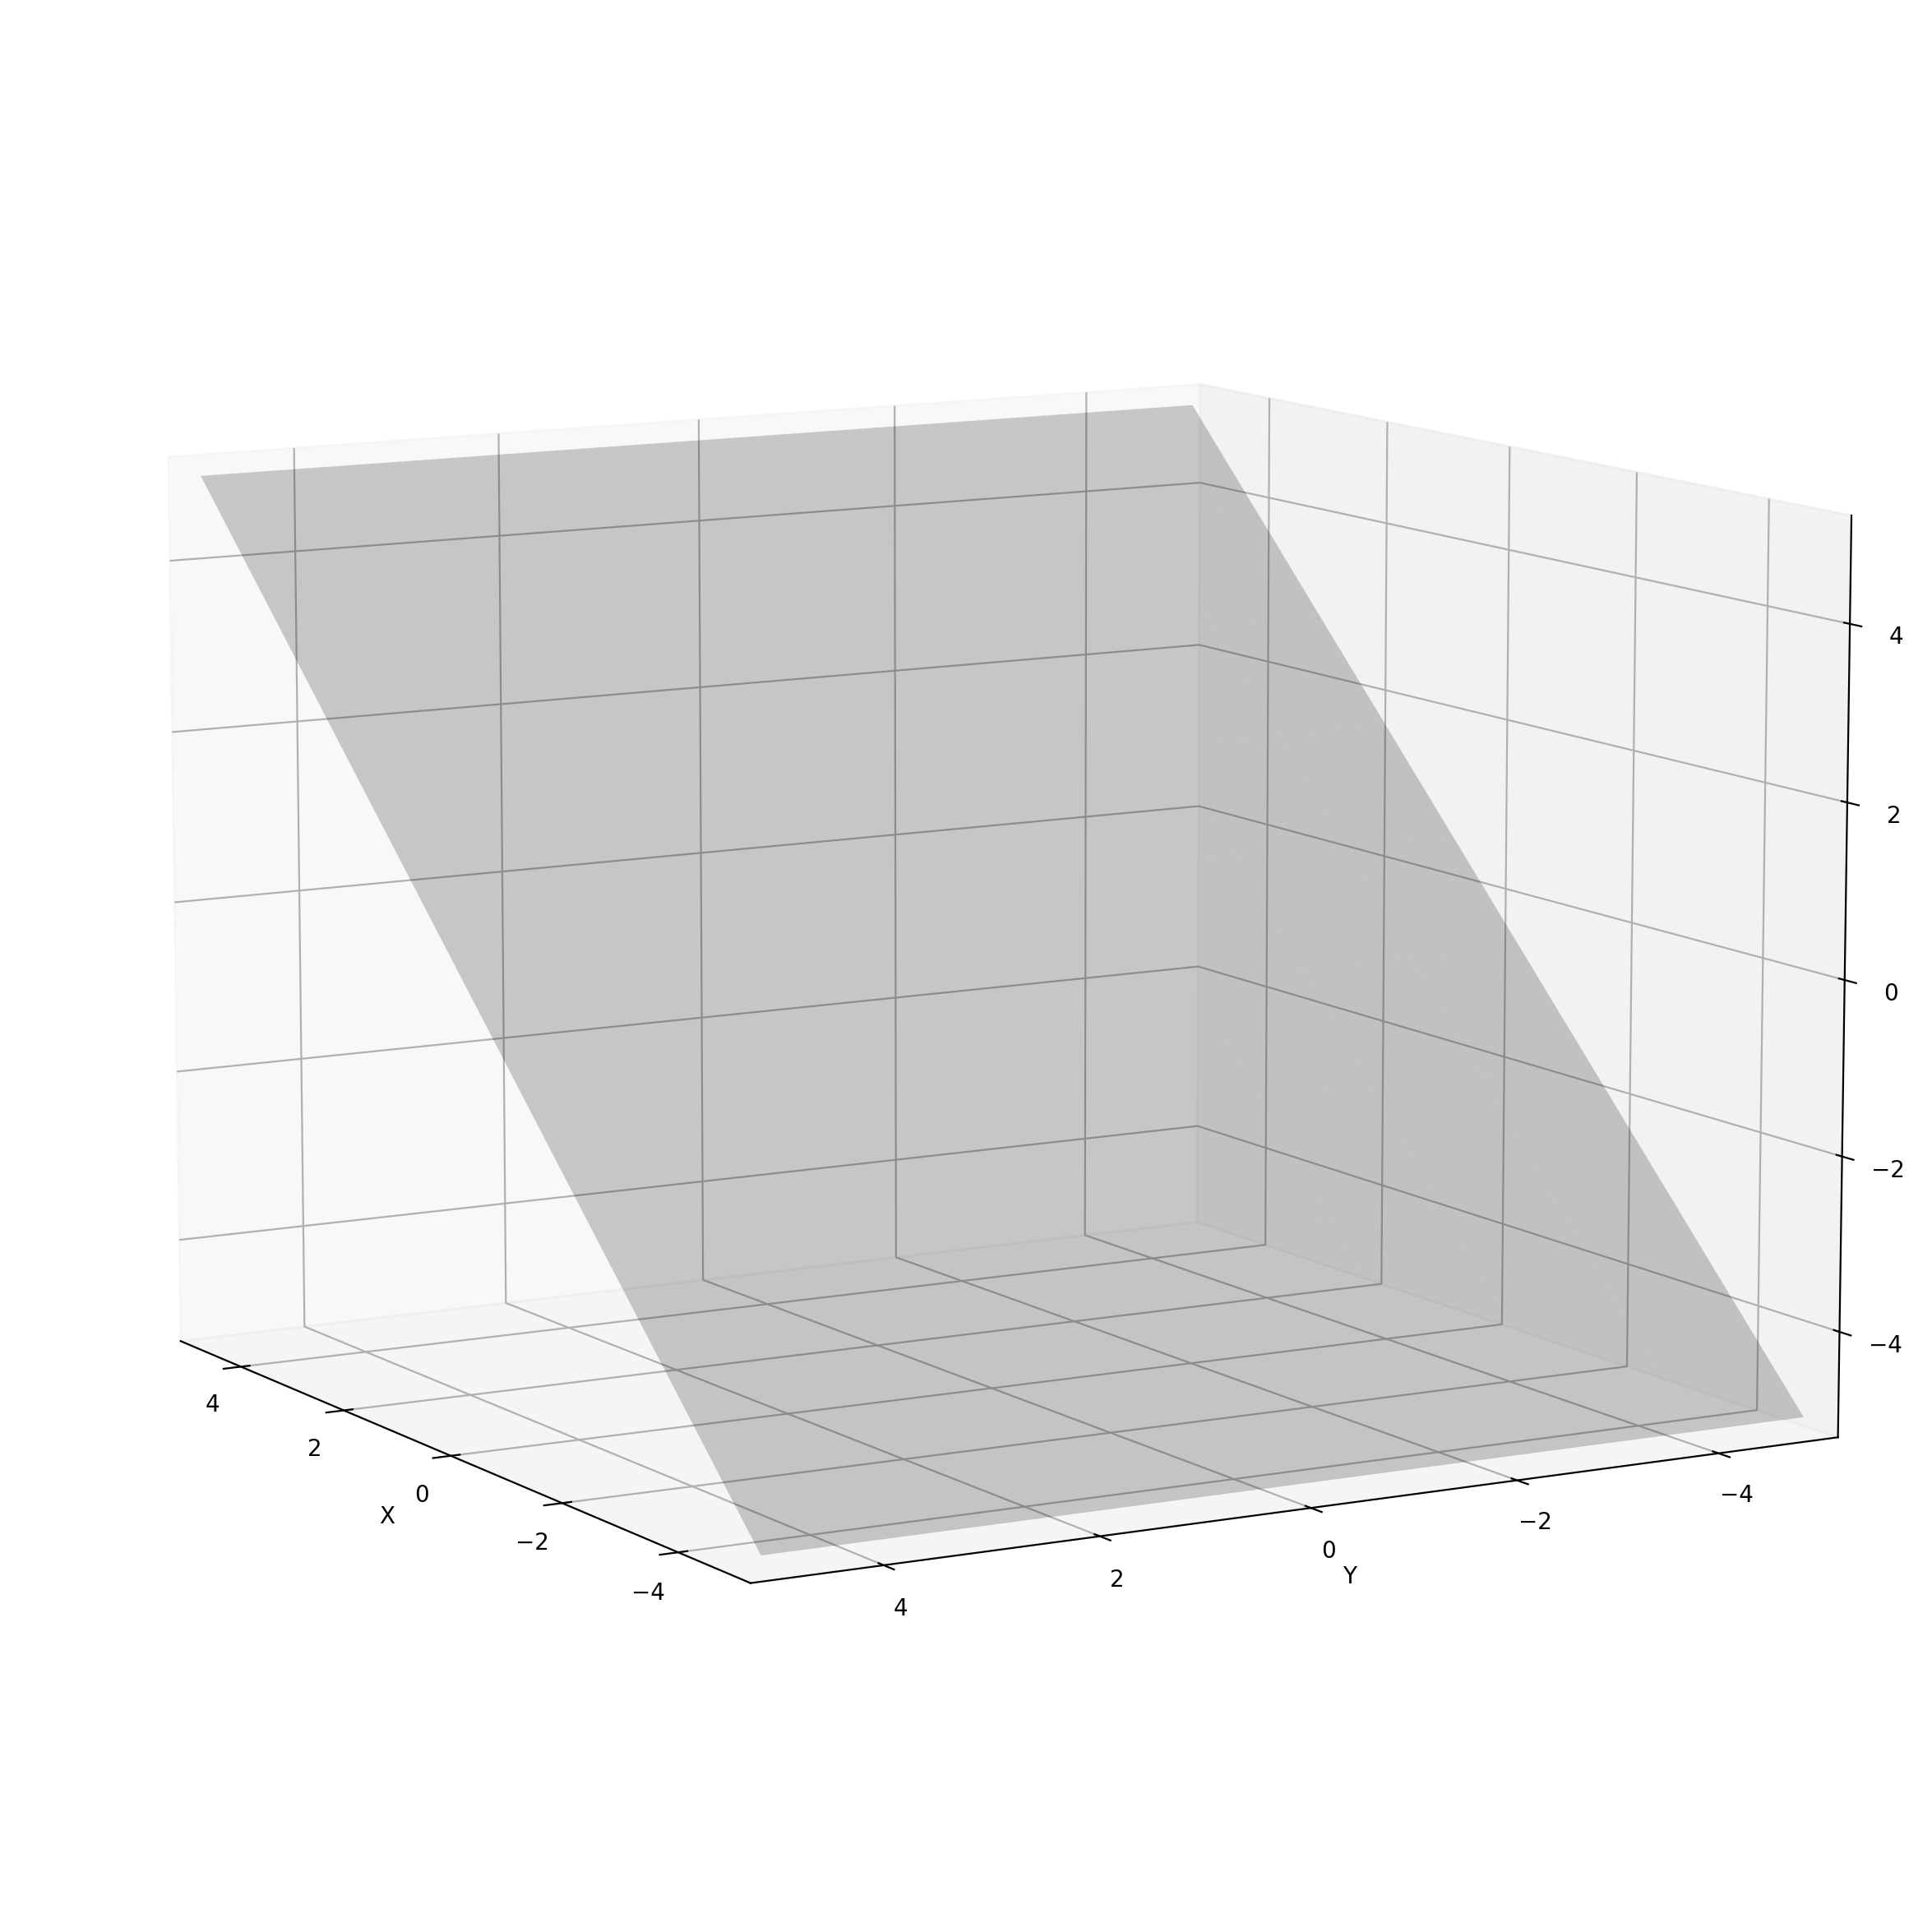
\includegraphics[scale=0.39]{Images/vector-space-ex.png}
    \caption{Graphical representation of $V$ vector space.}
    \label{fig:vector-space-ex}
\end{figure}

%%%%%%%%%%%%%%%%%%%%%%%%%%%%%%%%%%%%%%%%%%VECTOR-SUBSPACE%%%%%%%%%%%%%%%%%%%%%%%%%%%%%%%%%%%%%%%%%%%%%%%%%
\subsection{Vector Subspaces}

Let $V$ be a vector space over a field $\mathbb{F}$, and let $W$ be a non-empty subset of $V$. $W$ is called a \emph{vector subspace} of $V$ if it satisfies the following properties:

\begin{enumerate}
    \item \textbf{Closure under Vector Addition:} For any $\vec{u}, \vec{v} \in W$, their sum $\vec{u} + \vec{v}$ is also in $W$.
    
    \item \textbf{Closure under Scalar Multiplication:} For any $\vec{v} \in W$ and any scalar $c \in \mathbb{F}$, the scalar product $c\vec{v}$ is in $W$.
    
    \item \textbf{Contains the Zero Vector:} The zero vector $\vec{0}$ of $V$ is in $W$.
\end{enumerate}

If these conditions are met, $W$ is a vector subspace of $V$ and is denoted as $W \subseteq V$.
\\

\textbf{Example of Vector Subspace}

Consider \(W\) as a vector subspace of previously defined space \(V\):

$$
\scalebox{1.1}{$W \subseteq V = \{\vec v \in \mathbb{R}^3 \ | \ v_3 = v_1\}$}
$$$$
\scalebox{1.1}{$W = \{ \vec{w} \in \mathbb{R}^3 \mid w_3 = w_1 \land w_1 + w_2 = 0\}$}
$$

In other words, \(W\) consists of all vectors in \(\mathbb{R}^3\) whose component $w_3$ is equal to $w_1$ and $w_1$ and $w_2$ components sum to zero.
\\

Let's check the three conditions for \(W\) to be a vector subspace:

\begin{enumerate}
    \item \textbf{Closure under Addition:}
     \begin{itemize}
            \item Take \(\vec{v} =\begin{bmatrix} v_1 \\ -v_1 \\ v_1 \end{bmatrix}\) and \(\vec{w} =\begin{bmatrix} w_1 \\ -w_1 \\ w_1 \end{bmatrix}\) where \(\vec v, \vec w \in W \).
            \item Their sum \(\vec{v} + \vec{w} =\begin{bmatrix} v_1 + w_1 \\ -(v_1 + w_1) \\ v_1 + w_1 \end{bmatrix} = \vec z\) is also in \(W\) because \(z_2 = -z_1 \land z_3 = z_1\).
        \end{itemize}
        
    \item \textbf{Closure under Scalar Multiplication:}
     \begin{itemize}
            \item Take \(\vec{w} =\begin{bmatrix} w_1 \\ -w_1 \\ w_1 \end{bmatrix} \in W\) and \(k \in \mathbb{R}\).
            \item The scalar multiple \(k \cdot \vec{w} =\begin{bmatrix} kw_1 \\ -(kw_1) \\ kw_1 \end{bmatrix} = \vec z\) is also in \(W\) since \(z_1 = -z_2 \land z_3 = z_1\).
        \end{itemize}
    
    \item \textbf{Contains the Zero Vector:}
     \begin{itemize}
            \item The zero vector \(\vec{0} =\begin{bmatrix} 0 \\ 0 \end{bmatrix}\) is in \(W\) because \(z_1 = -z_2 \land z_3 = z_1\).
        \end{itemize}
\end{enumerate}
Therefore, \(W\) satisfies all conditions and is indeed a vector subspace of \(V\).
\\

The graphical representation of the vector subspace $W$ is a one-dimensional line as shown in Figure \ref{fig:vector-subspace-ex}.
\begin{figure}[h]
    \centering
    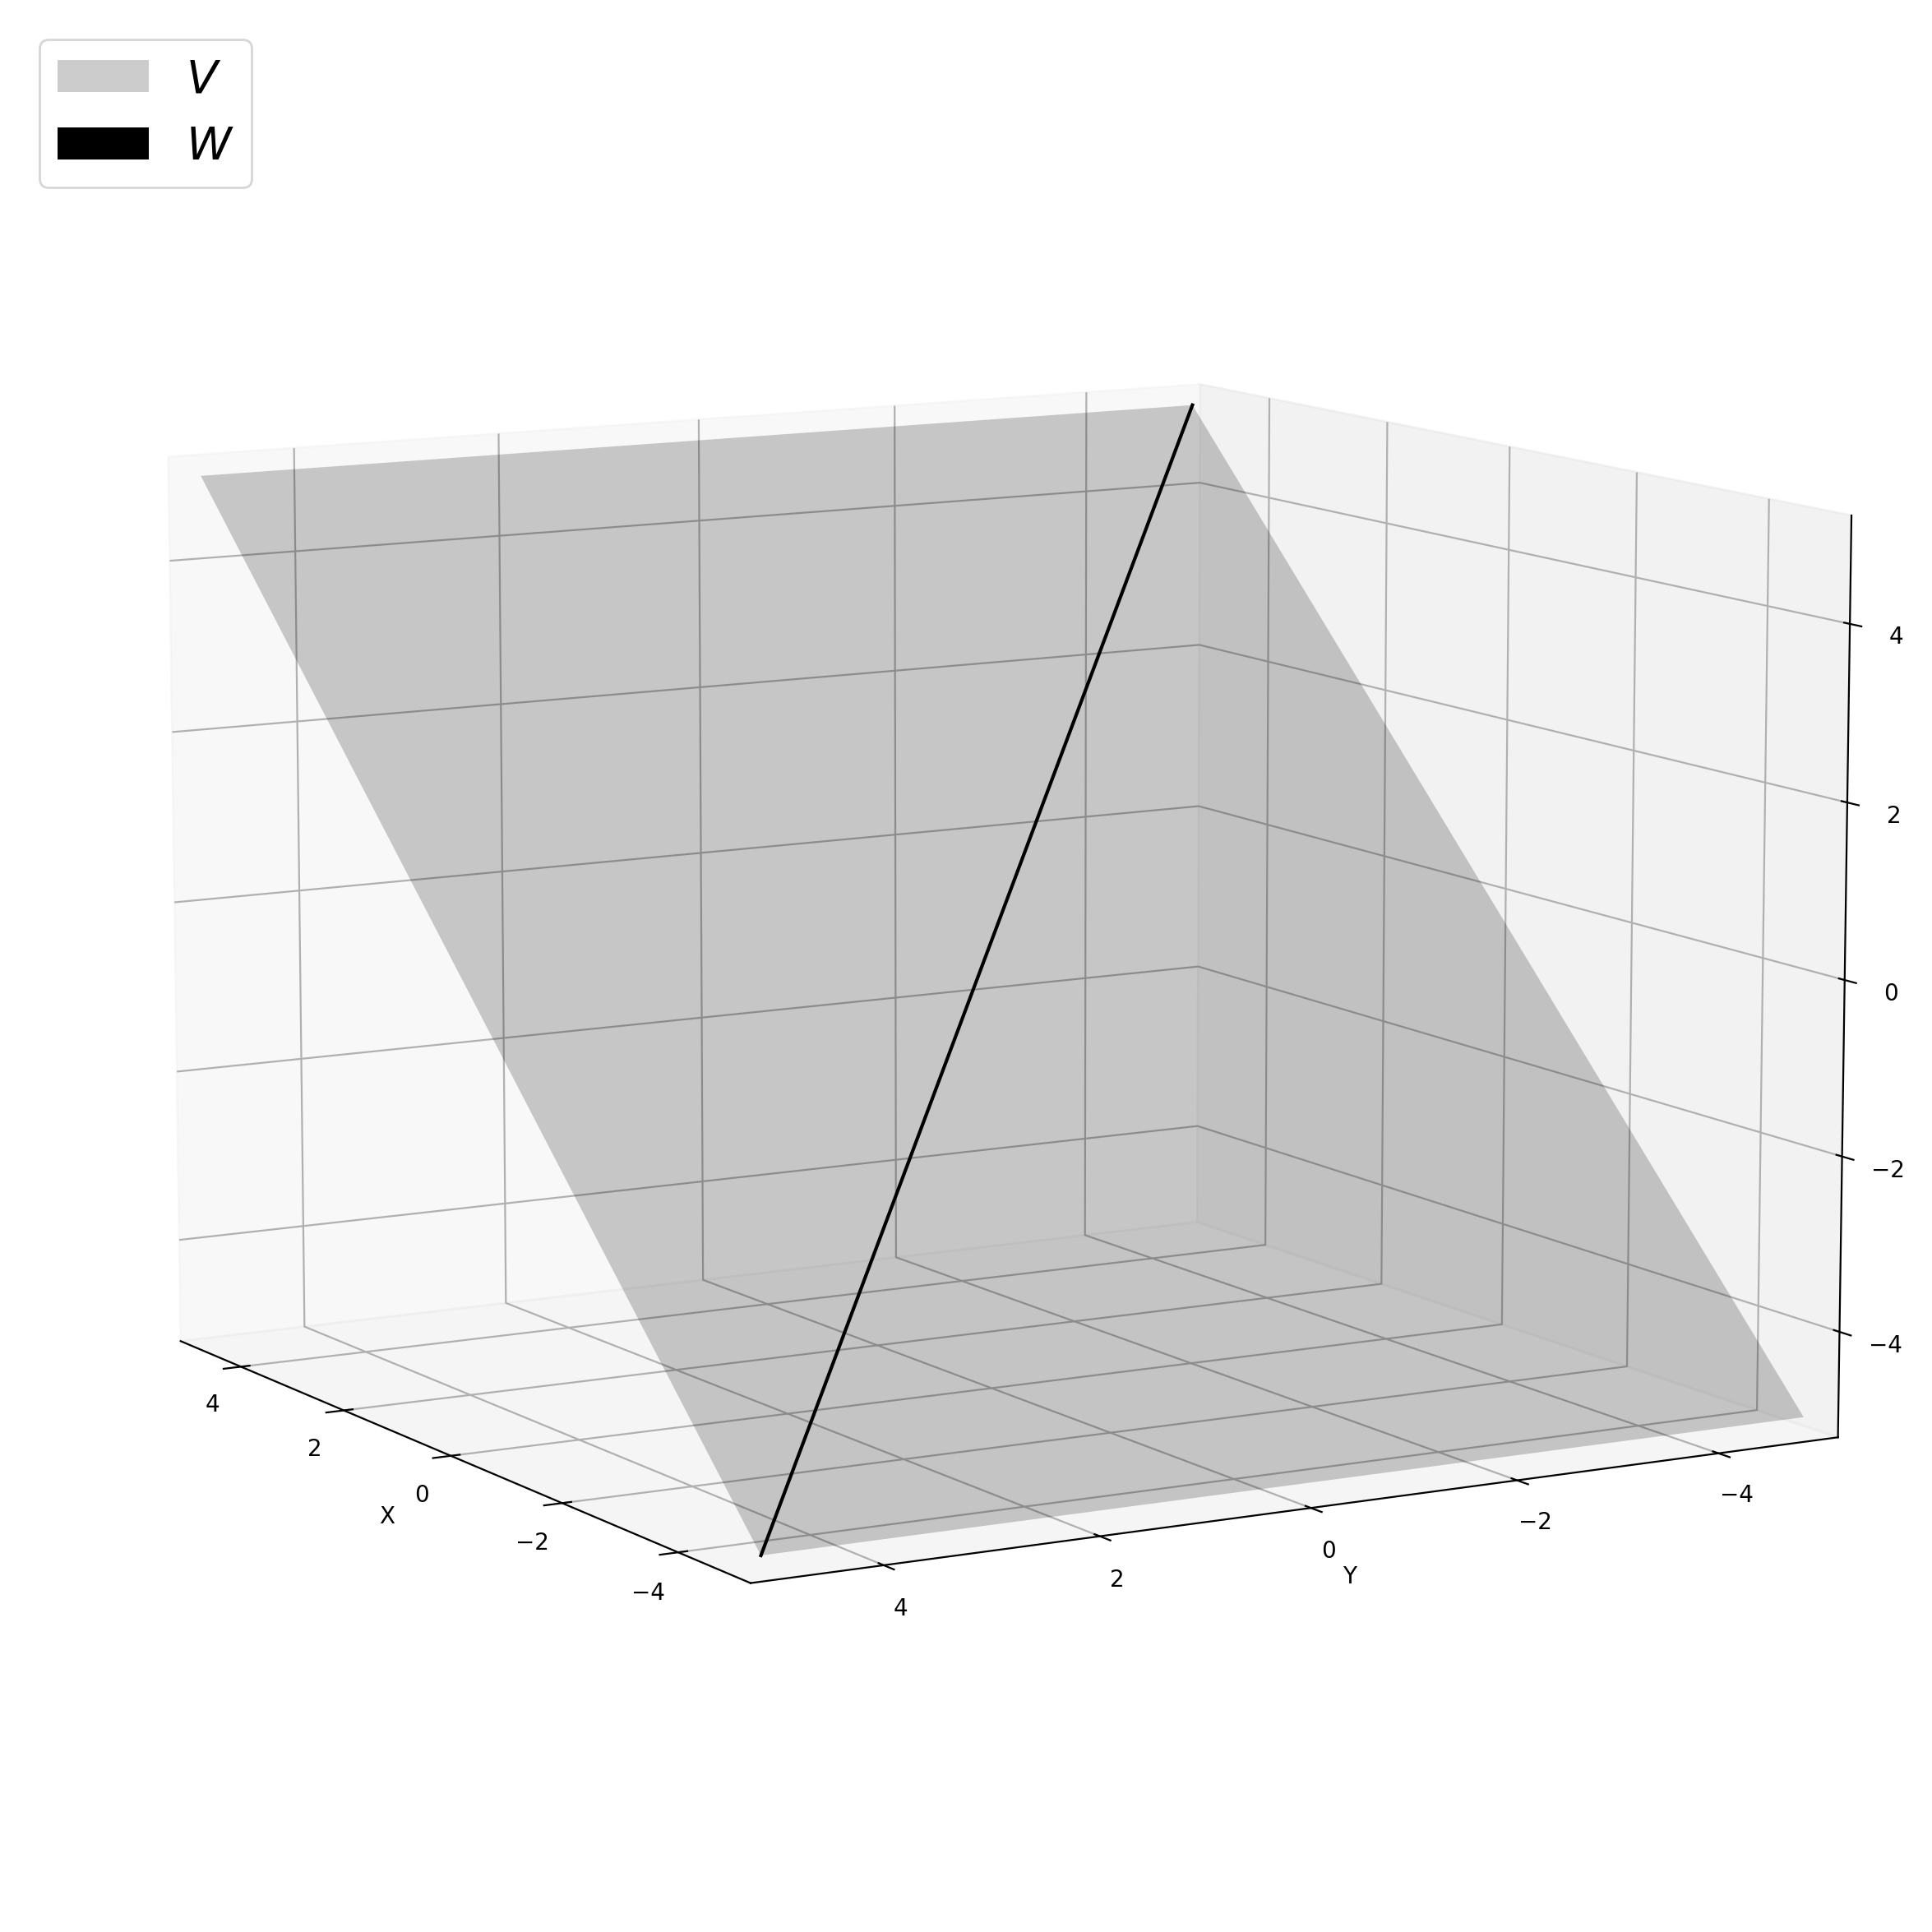
\includegraphics[scale=0.36]{Images/vector-subspace-ex.png}
    \caption{Graphical representation of $V$ vector space (gray) and $W$ vector subspace (black).}
    \label{fig:vector-subspace-ex}
\end{figure}

\subsubsection{Sum of Subspaces}

Let $U_1, \ldots, U_m$ be subspaces of $V$. The sum $U_1 + \cdots + U_m$ is a vector subspace of $V$, defined as the set of all possible sums of elements from $U_1, \ldots, U_m$, denoted by:

\[ U_1 + \cdots + U_m = \{ u_1 + \cdots + u_m : u_1 \in U_1, \cdots, u_m \in U_m \} \].

This sum represents the space formed by combining elements from each subspace. 
\\

The union of basis vectors (of each base) of each subspace is a spanning set for the new sum vector subspace $ U_1 + \cdots + U_m$.
\\

Note that if 

\begin{enumerate}
    \item $U_1 + \cdots + U_m = V$
    \item $U_1 \cap \cdots \cap U_m = \{\vec 0\}$
\end{enumerate}

The sum $U_1 + \cdots + U_m$ is called \textbf{direct sum} and it is denoted as

\[ U_1 \oplus \cdots \oplus U_m = \{ u_1 + \cdots + u_m : u_1 \in U_1, \ldots, u_m \in U_m\} \].

In a direct sum, every element of $U_1 \oplus \cdots \oplus U_m$ can be uniquely expressed as a sum $u_1 + \cdots + u_m$, where each $u_j$ belongs to $U_j$. And the only way to write 0 as a sum $u_1+...+u_m$ is by taking each $u_j$ equal to 0. So the union of the basis vectors (of each basis) of each vector space, form a basis for the new sum vector space.
\\

This represents a decomposition of the vector space $V$ into mutually exclusive subspaces, where each element has a unique representation as a sum of elements from the respective subspaces.
\\

%%%%%%%%%%%%%%%%%%%%%%%%%%%%%%%%%%%%%%%%Intersection-union%%%%%%%%%%%%%%%%%%%%%%%%%%%%%%%%%%%%%%%%%%%%
\subsubsection{Intersection of Subspaces}

Consider subspaces $V$ and $W$ of a vector space $U$. The intersection $V \cap W$ is also a subspace of $U$.

Since both $V$ and $W$ are subspaces, they contain the zero vector, making $V \cap W$ nonempty. Let $\vec v_1, \vec v_2 \in V \cap W$. As $V$ and $W$ are closed under addition, $\vec v_1 + \vec v_2 \in V$ and $\vec v_1 + \vec v_2 \in W$, implying $\vec v_1 + \vec v_2 \in V \cap W$. Thus, $V \cap W$ is closed under addition.

Consider $c \in \mathbb{R}$ and $v \in V \cap W$. Since $V$ and $W$ are closed under scalar multiplication, $c \vec v \in V$ and $c \vec v \in W$, indicating $c \vec v \in V \cap W$. Therefore, $V \cap W$ is closed under scalar multiplication.

These closures demonstrate that the intersection of subspaces preserves the subspace property within the overarching vector space $U$.

\subsubsection{Union of Subspaces}

In contrast, the union of subspaces $V$ and $W$ may not form a subspace of $U$. For instance, consider two distinct lines passing through the origin in $\mathbb{R}^2$. While each line individually forms a subspace, their union lacks closure under addition, failing to be a subspace.
%%%%%%%%%%%%%%%%%%%%%%%%%%%%%%%%%%%%%%%%LINEAR-COMBINATIONS%%%%%%%%%%%%%%%%%%%%%%%%%%%%%%%%%%%%%%%%%%%%%%%%%%%%%
\section{Linear Combinations}

In the realm of vector spaces, the concept of a \emph{linear combination} holds significant importance. A \emph{linear combination} involves combining vectors in a space by scaling each vector by a scalar and then summing them up. 


    Let $V$ be a vector space over the field $\mathbb F$. If $\vec{v}_1, . \ . \ ., \vec v_s \in V$ are vectors and $a_1, . \ . \ ., a_s \in \mathbb F$ are scalars, then the \textbf{linear combination} of those vectors with those scalars as coefficients is 

$$
a_1 \vec v_1 + \dots + a_s \vec v_s \ \in V, \quad a_1, . \ . \ ., a_s \in \mathbb F.
$$

\label{def:linear-combination}

Understanding linear combinations is foundational in linear algebra, providing insights into the structure and properties of vector spaces. Linear combinations play a crucial role in defining concepts such as span, linear independence, and solutions to systems of linear equations.
%%%%%%%%%%%%%%%%%%%%%%%%%%%%%%%%%%%%%%%%%%SPAN%%%%%%%%%%%%%%%%%%%%%%%%%%%%%%%%%%%%%%%%%%%%%%%%%
\subsection{Span}

The \textbf{span} of a nonempty subset $S$ of a vector space $V$ over a field $\mathbb F$, is the set of all possible linear combinations of those vectors.

$$
\textit{span}(\vec{v}_1, \vec{v}_2, \ldots, \vec{v}_k) = \left\{ \sum_{i=1}^k \lambda_i \vec{v}_i \ \middle| \ k \in \mathbb{N}, \vec{v}_i \in V, \lambda_i \in \mathbb F \right\}
$$

The span of the empty subset of a vector space is its trivial subspace.
\\

In simpler terms, the span is the set of all possible vectors that can be formed by linear combinations of the given vectors.
\\

Let $S \subseteq V$. The set $S$ is a \textbf{spanning set} of $V$ if \textit{every} $\vec v \in V$ can be written as linear combination of vectors in $S$.


\subsubsection{The Span of a Subset of a Vector Space is a Vector Subspace}

Let $S$ be a set of vectors of vector space $V$. The {\textit{span($S$)}} is a vector subspace.
\\

It is easy to show that the span of $S$ contain the $\vec 0$ and is closed under addition and scalar multiplication.

All the other axioms are inherited from $V$.
\\

The span plays a crucial role in determining the extent or reach of a set of vectors. If the span of a set of vectors is the entire vector space $V$, then the vectors are said to \emph{span} the space.
%%%%%%%%%%%%%%%%%%%%%%%%%%%%%%%%%%%%%%%%%%LINEAR-INDEPENDENCE%%%%%%%%%%%%%%%%%%%%%%%%%%%%%%%%%%%%%%%%%%%%%%%%%
\section{Linear (in)dependence}

In a vector space $V$, a subset of vectors is deemed \emph{linearly independent} if no vector within the subset can be expressed as a linear combination of others in the same subset. Conversely, if such a linear combination exists, the subset is \emph{linearly dependent}.
\\

Now, let's explore some implications of these definitions!
\\

Consider a subset $S$ of vectors in a vector space $V$. If $S$ is linearly independent, then the only way to obtain the zero vector through a linear combination of its elements is by using all coefficients as zero:

$$
c_1 \vec s_1 + \dots +, c_n \vec s_n = \vec 0, \quad \text{with} \ \ c_1 = \dots = c_n = 0 .
$$

This condition serves as a hallmark of linear independence.
\\

Conversely, if a subset $S$ is not linearly independent, it implies the existence of at least one vector that can be expressed as a linear combination of the others. For example the vector 

$$
\vec s_i = c_1 \vec s_1 + \dots + c_{i-1} \vec s_{i-1} + c_{i+1} \vec s_{i+1} + \dots + c_n \vec s_n,
$$

is linearly dependent from vectors in $\{\vec s_1, \dots, \vec s_{i-1}, \vec s_{i+1}, \dots, \vec s_n\}$.

In this case, the subset $\{\vec s_1, \dots, \vec s_n\}$ is termed linearly dependent. This dependence is evident when one of the vectors can be obtained by combining the rest.
\\

Furthermore, the span of a subset of vectors in a vector space, denoted as $span(S)$, encompasses all possible linear combinations of the vectors in $S$. Interestingly, the span itself forms a vector subspace of $V$, regardless of the choice of subset $S$. This property underscores the structural coherence of vector spaces under linear combinations.
\\

Moreover, adding a vector $\vec{v}$ to a set $S$ expands its span only if $\vec{v}$ is not already in the span of $S$. Conversely, removing a vector from a set $S$ shrinks its span if and only if the removed vector was not a linear combination of the others. In both this cases, the vector $\vec v$ is linearly independent from vectors in $S$. This observation leads to a significant corollary: in any vector space, every finite set of vectors possesses a linearly independent subset with the same span.
\\

Additionally, the removal of a vector from a linearly independent set preserves its linear independence. Conversely, any superset of a linearly dependent set inherits its linear dependence. These observations highlight the robustness of linear independence and dependence under subset and superset operations.
%%%%%%%%%%%%%%%%%%%%%%%%%%%%%%%%%%%%%%%%%%BASIS%%%%%%%%%%%%%%%%%%%%%%%%%%%%%%%%%%%%%%%%%%%%%%%%%
\section{Basis and Dimension}

\subsection{Basis}

A maximal linearly independent subset of vectors of $V$ that spans $V$ is called a \textbf{basis} of the vector space $V$.
\\

This means that a subset $B$ of $V$ is a \textbf{basis} if it satisfies the two following conditions:

\begin{itemize}
\item \textbf{Linear independence:}
    For every finite subset $\{ \vec{\beta} _{1},\dotsc ,\vec {\beta}_{n}\}$ of $B$, if ${\displaystyle c_{1}\vec {\beta}_{1} + \cdots + c_{n}\vec {\beta}_{n}=\vec {0} }$ for some ${\displaystyle c_{1},\dotsc ,c_{m}}$ in $\mathbb F$, then ${\displaystyle c_{1}=\cdots =c_{m}=0}$.
\item \textbf{Spanning property:}
    For every vector $\vec{v}$ in $V$, one can choose ${\displaystyle a_{1},\dots, a_{n}}$ in $\mathbb F$ and ${\displaystyle \vec {\beta}_{1},\dots  ,\vec {\beta}_{n}}$ in $B$ such that ${\displaystyle \vec {v} = a_{1}\vec {\beta}_{1} + \cdots + a_{n}\vec {\beta}_{n}}$.
\end{itemize}

The scalars $a_{i}$ are called the coordinates of the vector $\vec{v}$ with respect to the \textbf{basis} $B$, and by the first property they are uniquely determined.
\\

Note that is more useful to consider a basis as a sequence of vectors instead of a set. This because when considering the coordinates of a vector, we have an implicit need to know the order of the basis vectors for applying coordinates to the right basis vectors. For this reason, we will denote a basis with angle brackets $\langle \beta_1, \beta_2, \dots, \beta_n \rangle$.
\\

In a vector space $V$ with a basis $B = \langle\vec \beta_1, \dots, \vec \beta_n \rangle$, the coordinates of a generic vector $\vec v \in V$ are the coefficients used to express $\vec v$ as a linear combinations of the basis vectors. So the coordinates of the vector $\vec v \in V$ with respect to basis $B$ are represented by the column vector 

$$
[ \ \vec v \ ]_B =\begin{bmatrix}
    c_1 \\
    \vdots\\
    c_n
\end{bmatrix}
$$



In a vector space, the coordinates of a vector with respect to a given \emph{basis} are unique. Specifically, let $V$ be a vector space and $B = \langle \vec{\beta}_1, \vec{\beta}_2, \ldots, \vec{\beta}_n\rangle$ be a \emph{basis} for $V$. For any vector $\vec{v} \in V$, there exists a unique set of scalars $c_1, c_2, \ldots, c_n$ such that:

$$
\vec{v} = c_1 \vec{\beta}_1 + c_2 \vec{\beta}_2 + \ldots + c_n \vec{\beta}_n
$$

This uniqueness property ensures that the coordinates of $\vec{v}$ in terms of the \emph{basis} $B$ are well-defined and distinct.
\\

We can view a basis of a vector space as a minimal subset of vectors with which we can control all the dimensions of a vector space. In particular, each vector in the basis is responsible for "controlling" one dimension of the vector space. This way, through coefficients, we can express each dimension of the vector space. From the perspective of an individual component of a vector: the basis vector responsible for the $i$-th component of vector $\vec{v}$ will be a vector from the basis (let's denote it for simplicity as $\vec{\beta}_x \in B$). In this case, the $i$-th component of the basis vector $\vec{\beta}_x$ and the coefficient $\alpha_x$ will be responsible for generating the $i$-th component of vector $\vec{v}$ in a similar way to this: $v_i = \alpha_x b_{x_i}$.
\\

However, since there are other combinations that indirectly affect the same dimension managed by the basis vector $\vec{\beta}_x$, we also need to include these coefficients in the equation. Thus, we obtain $v_i = \alpha_1 \vec\beta^i_{1} + \ldots + \alpha_x \vec{\beta}^i_{x} + \ldots + \alpha_n \vec{\beta}^i_{n}$. Therefore, to find all the coefficients of the basis for vector $\vec{v}$ (across all components), one needs to solve the linear system $v_i = \alpha_1 \vec{\beta}^i_{1} + \ldots + \alpha_x \vec{\beta}^i_{x} + \ldots + \alpha_n \vec{\beta}^i_{n}$ for each $i$ from $1$ to $n$.

$$
\begin{cases}
\alpha_1 \vec{\beta}^{\ 1}_{1} + \ldots + \alpha_x \vec{\beta}^{\ 1}_{x} + \ldots + \alpha_n \vec{\beta}^{\ 1}_{n} = v_1 \\
\ \ \vdots\\
\alpha_1 \vec{\beta}^{\ n}_{1} + \ldots + \alpha_x \vec{\beta}^{\ n}_{x} + \ldots + \alpha_n \vec{\beta}^{\ n}_{n} = v_n
\end{cases}
$$

And since it is a linear system of $n$ equations and $n$ variables (where all equations are linearly independent, as we mentioned that ${B}$ is a minimal set that can control all dimensions of $V$), we obtain a unique solution for each vector in $V$.


For each $\mathbb{R}^n$ vector space, the vectors 

$$\xi_n = \langle \begin{bmatrix} 1 \\ 0 \\ 0 \\ \vdots \\ 0\end{bmatrix}, \\ \begin{bmatrix} 0 \\ 1 \\ 0 \\ \vdots \\ 0\end{bmatrix}, \ \dots, \\\begin{bmatrix} 0 \\ 0 \\ 0 \\ \vdots \\ 1\end{bmatrix}\rangle$$ 

are a \textbf{basis} (known as \emph{canonical} \textbf{basis}) also known as $\xi_n$. We denote these vectors $\vec{e}_1, \dots, \vec{e}_n$.
\\

Every non-trivial vector space posses a basis. The trivial one, instead, doesn't have a basis (its basis is $\emptyset$). Existence of a basis in a vector space is guaranteed by the properties of spanning and linear independence.
\\

For a given basis $B$ of $V$ with $n$ elements, a linear combination of vectors $a_1 \vec v_1 + \cdots + a_k \vec v_k= \vec 0$ if and only if $a_1 [\vec v_1]_B + \cdots + a_k [\vec v_k]_B = \vec 0$.
\\

In fact, let $\langle \vec \beta_1, \cdots, \vec \beta_n \rangle$ be a basis of $V$ vector space. Each vector $\vec v_i \in V$ can be expressed as a linear combination of basis vector, so:

\begin{align*}
a_1 \vec v_1 + \cdots + a_k \vec v_k &= a_1 (\alpha_{1,1} \vec \beta_1 + \cdots + \alpha_{1,n} \vec \beta_n) + \cdots + a_k (\alpha_{k,1} \vec \beta_1 + \cdots + \alpha_{k,n} \vec \beta_n) = \\
&=(a_1 \alpha_{1,1} + \cdots + a_k \alpha_{k,1}) \vec \beta_1 + \cdots + (a_1 \alpha_{1,n} + \cdots + a_k \alpha_{k,n}) \vec \beta_n = \vec 0.
\end{align*}

This implies that

$$
\begin{cases}
a_1 \alpha_{1,1} + \cdots + a_k \alpha_{k,1} = 0 \\
\ \ \vdots\\
a_1 \alpha_{1,n} + \cdots + a_k \alpha_{k,n} = 0
\end{cases}
$$

that can be easily written as follow:

$$
a_1 \begin{bmatrix}
\alpha_{1,1}\\
\vdots\\
\alpha_{1,n}
\end{bmatrix} + \cdots + a_{k} \begin{bmatrix}
\alpha_{k,1}\\
\vdots\\
\alpha_{k,n}
\end{bmatrix}
= a_1 [\vec v_1]_B + \cdots + a_k [\vec v_k]_B = \vec 0.
$$

Geometrically, the whole matter can be interpreted in this way: each coordinate vector of every vector in the initial linear combination is "telling" how much "force" to apply to each base vector that "controls" a certain coordinate. Let's take an example: consider a generic component of every vector in the initial combination. We know that the combination $a_1 v_i + \cdots + a_k v_i$ equals zero, which tells us that the forces acting on the $i$-th component of the combination cancel out. However, this component (and all other components) stem from a sum of a linear combination of the $i$-th components of the base vectors. This implies that the force applied to any generic component is equally expressed by the same base vectors. So, for example $6=3\cdot2$ and $3=3\cdot1$, the combination $2 \cdot 6 + (-4) \cdot 3 = 0$, so also $2 \cdot (3\cdot2) + (-4) \cdot (3\cdot1) = 0$; now you can note that the number $3$ is our basis number, it can express $3$ and $6$.
The coordinate of $6$ is $2$ and the coordinate of $3$ is $1$. Substitute now $6$ with $3$ and $3$ with $1$ in the first combination and tah dah: $2 \cdot 2 + (-4) \cdot 1 = 0$. That is obvious because we have scaled the \textbf{same} basis number by two factors that cancel each other out.
\\

\textbf{Steinitz Lemma}\\
This lemma describes a relationship between the sizes of linearly independent sets and spanning sets within a vector space. It states that if you have a linearly independent set $U$ and a spanning set $W$ in a vector space $V$, then the size of $U$ cannot exceed the size of $W$. Furthermore, it asserts that by removing a specific number of vectors from $W$, you can create a new set that, when combined with $U$, still spans the entire space $V$. This lemma highlights the balance between linear independence and spanning capabilities in constructing bases for vector spaces.

This lemma can be understood in terms of spanning and linear independence in vector spaces. Imagine a vector space as a geometric plane or higher-dimensional space. A set of vectors is linearly independent if none of them can be expressed as a linear combination of the others. This implies that each vector in the set contributes a unique direction to the space. On the other hand, a spanning set encompasses vectors that collectively cover the entire space, allowing you to reach any point within it through linear combinations of those vectors.

The Steinitz Lemma highlights a balance between these two aspects: linear independence and spanning capability. It states that if you have a set of vectors that are linearly independent and another set that spans the space, you cannot have more linearly independent vectors than those that span the space. In other words, you can't introduce more unique directions than necessary to cover the entire space. Moreover, the lemma suggests that you can fine-tune the spanning set by removing redundant vectors while still ensuring that it covers the space adequately.
\\

\textbf{Exchange Lemma}\\
This lemma addresses the process of exchanging vectors within a basis while maintaining the basis' fundamental properties. It states that given a vector space $V$ and a basis $B$, if there exists a vector $\vec{v}$ that can replace one of the basis vectors while preserving linear independence, then the resulting set after the exchange still forms a basis for $V$. This lemma offers an intuitive understanding of how bases can be modified without compromising their essential properties. Think of a basis as a set of vectors that serves as the "building blocks" for constructing any vector within the space through linear combinations. The Exchange Lemma states that if you have a basis and you encounter a vector that can replace one of the basis vectors while preserving linear independence, you can make that exchange without losing the ability to represent all vectors in the space.

Geometrically, this means that if you have a set of vectors forming a basis, each vector contributes a unique direction to the space. If you find another vector that can take the place of one of the basis vectors without introducing any redundant direction, you can seamlessly integrate it into the basis. This process allows for flexibility in choosing basis vectors while ensuring that the resulting set still forms a complete "framework" for the vector space.
\\


\textbf{Theorem on Basis Size Consistency}\\
This theorem establishes a fundamental property of bases in finite-dimensional vector spaces. It asserts that all bases of a finite-dimensional vector space have the same number of elements. In other words, the size of a basis is an intrinsic property of the vector space itself and does not depend on the specific choice of basis vectors. This theorem underscores the uniformity and consistency of bases across a given vector space.

Geometrically, this theorem reflects the uniformity of bases across a given vector space. Imagine a basis as a set of vectors that forms the "standard directions" or "axes" along which you can measure and describe vectors within the space. The theorem asserts that, regardless of the specific choice of basis vectors, the number of these "standard directions" remains constant for a finite-dimensional vector space.

In essence, this theorem emphasizes the intrinsic properties of vector spaces that dictate the number of dimensions needed to describe them fully. It implies that the dimensionality of a space is a well-defined characteristic that transcends the individual choice of basis vectors, highlighting the consistency and universality of bases within the same vector space.

\subsection{Dimension}

The \emph{dimension} of a vector space is a fundamental concept that quantifies the "size" or "degree of freedom" of the space. For a vector space $V$, the dimension is defined as the  the cardinality of a basis of $V$. The \emph{dimension} of the trivial vector space is equal to 0, since its basis is $\emptyset$.
\\

A vector space $V$ with a basis $B$ is \emph{finite-dimensional} if the basis $B$ has finitely many vectors
\\

\textbf{Dimensionality Corollary: Limits of Linear Independence}\\
The corollary regarding the dimension of linearly independent sets states that in a vector space, the maximum number of linearly independent vectors within a set is bounded by the dimensionality of the space. This implies that adding more vectors beyond this limit leads to linear dependence, compromising the independence of the set. 
\\

Geometrically, it signifies that in a space of a given dimension, there is a finite capacity for representing distinct directions or degrees of freedom with linearly independent vectors. Algebraically, it underscores the role of dimensionality as an upper bound for the size of independent sets, reflecting the inherent structure of the space. This corollary guides the analysis of systems of equations, subspaces, and transformations by providing insight into the relationship between linear independence and space dimension. 
\\

Ultimately, it illuminates the fundamental connection between the structure of vector spaces and the properties of their subsets, offering a foundational principle for mathematical reasoning and analysis.
\\

\textbf{Dimensionality Corollary: Minimum Spanning Sets}\\
The corollary states that any spanning set in a vector space must contain at least as many vectors as the dimension of the space. In a vector space of dimension $n$, a spanning set cannot have fewer than $n$ vectors. This is because a spanning set must be able to generate all vectors within the space. If it had fewer than $n$ vectors, there would not be enough basis vectors to span the entire space. Thus, the minimum size of a spanning set is the dimension of the vector space. 
\\

This corollary highlights a fundamental property of spanning sets: they must have sufficient vectors to cover the entire space, ensuring that any vector in the space can be expressed as a linear combination of those spanning vectors. It underscores the relationship between the dimension of a vector space and the minimum number of vectors required to span that space effectively.
\\

\textbf{Interconnection of Linear Independence and Spanning Sets in Vector Spaces}\\
Combining the two previous results yields a fundamental understanding of linear independence and spanning sets in a vector space. The first corollary establishes that the maximum number of linearly independent vectors within a set is bounded by the dimensionality of the vector space. It implies that exceeding this limit results in linear dependence, compromising the set's independence. 

Conversely, the second result, the theorem, states that any spanning set must contain at least $n$ vectors in a vector space of dimension $n$. If it had fewer than $n$ vectors, there would not be enough vectors to span the entire space.

Therefore, the duality between linear independence and spanning sets is clear: a set of $n$ linearly independent vectors is guaranteed to span a space of dimension $n$, while a spanning set with $n$ vectors ensures linear independence and sufficiency for spanning the space. This interconnection underscores the importance of these concepts in understanding the structure and properties of vector spaces.
\\

\textbf{Dimension Inequality}\\
If \(V\) is finite-dimensional and \(U\) is a subspace of \(V\), then \(\text{dim} \, U \leq \text{dim} \, V\). This inequality highlights that the dimension of a subspace cannot exceed the dimension of its parent vector space.
\\

Geometrically, this statement reflects the idea that a subspace cannot "stick out" beyond the dimensions of its parent space. If you imagine a three-dimensional room (parent space) and a two-dimensional wall within it (subspace), the wall cannot extend beyond the boundaries of the room. Therefore, the dimension of the subspace must be less than or equal to the dimension of the parent space.
\\

\textbf{Equality of Dimensions}\\
Suppose \(V\) is finite-dimensional and \(U\) is a subspace of \(V\) such that \(\text{dim} \, U = \text{dim} \, V\). Then \(U = V\). This equality asserts that when the dimensions of a subspace and its parent space are equal, the subspace spans the entire parent space.
\\

This concept can be visualized as a smaller room (subspace) filling up the entire space of a larger room (parent space). If both rooms have the same dimensions, it means the smaller room perfectly fits within the larger one, occupying all available space. Geometrically, this represents a complete overlap between the subspace and the parent space.
\\

\textbf{Dimension of Sum of Subspaces}\\
For subspaces \(V_1\) and \(V_2\) of a finite-dimensional vector space, \(\text{dim}(V_1 + V_2) = \text{dim} \, V_1 + \text{dim} \, V_2 - \text{dim}(V_1 \cap V_2)\). This equation determines the dimension of the sum of two subspaces based on their individual dimensions and their intersection.
\\

Geometrically, this theorem describes how the dimensions of subspaces interact when they are combined. It's like stacking two rooms (subspaces) on top of each other within a building (parent space). The combined space's dimension is determined by adding the individual dimensions of each room and then adjusting for any shared areas between them. This reflects the total usable space created by the combination of both subspaces.
\\
\section{Rows and Columns Space}

In this section, we will investigate the vector space spanned by the row vectors (or column vectors) of a matrix. And, in the next chapter, we will see how such spaces relate to solutions of systems of linear equations.

To begin, you need to know some terminology. For an $m \times n$ matrix 

\[
A = \begin{bmatrix}
a_{1,1} & a_{1,2} & \dots & a_{1,n} \\
a_{2,1} & a_{2,2} & \dots & a_{2,n} \\
\vdots & \vdots & \ddots & \vdots \\
a_{m,1} & a_{m,2} & \dots & a_{m,n} \\
\end{bmatrix},
\]

the $n$-tuples corresponding to the rows of $A$ are called the row vectors of $A$.


\textbf{Row Vectors of $A$:}
\[
\begin{aligned}
& \vec r_1 = \begin{pmatrix} a_{1,1}, & a_{1,2}, & \dots, & a_{1,n} \end{pmatrix} \\
& \vec r_2 = \begin{pmatrix} a_{2,1}, & a_{2,2}, & \dots, & a_{2,n} \end{pmatrix} \\
&  \ \quad \quad \quad \quad \quad \vdots \\
& \vec r_m = \begin{pmatrix} a_{m,1}, & a_{m,2}, & \dots, & a_{m,n} \end{pmatrix}
\end{aligned}
\]

Similarly, the columns of $A$ are called the column vectors of $A$. You will find it useful to preserve the column notation for these column vectors.

\textbf{Column Vectors of $A$:}
\[
\begin{aligned}
& \vec c_1 = \begin{pmatrix} a_{1,1} \\ a_{2,1} \\ \vdots \\ a_{m,1} \end{pmatrix} \quad
\begin{pmatrix} a_{1,2} \\ a_{2,2} \\ \vdots \\ a_{m,2} \end{pmatrix} \quad
\dots \quad
\begin{pmatrix} a_{1,n} \\ a_{2,n} \\ \vdots \\ a_{m,n} \end{pmatrix}
\end{aligned}
\]

Two fundamental concepts associated with matrices are the row space and column space, which offer deep insights into their structure and behavior.

Consider a matrix $A$ with dimensions $m \times n$. The row space of $A$, denoted as $\text{Row}(A)$, encompasses all possible linear combinations of its row vectors. Mathematically, it can be represented as the subspace spanned by the row vectors of $A$ in $\mathbb{R}^n$. 

Formally:

\[
\text{Row}(A) = \text{span}\{\vec{r}_1, \vec{r}_2, \ldots, \vec{r}_m\}
\]

where $\vec{r}_i$ represents the $i$-th row vector of $A$.

Similarly, the column space of $A$, denoted as $\text{Col}(A)$, captures all possible linear combinations of its column vectors. It forms a subspace spanned by the column vectors of $A$ in $\mathbb{R}^m$. 

Formally:

\[
\text{Col}(A) = \text{span}\{\vec{c}_1, \vec{c}_2, \ldots, \vec{c}_n\}
\]

where $\vec{c}_i$ represents the $i$-th column vector of $A$.

\subsection{Row-Equivalent Matrices and Row Space}

The row space of a matrix refers to the space formed by all possible linear combinations of its row vectors. Two matrices are considered row-equivalent if one can be obtained from the other through elementary row operations, such as multiplying a row by a number or adding one row to another. 

If matrix A can be turned into matrix B through these operations, then the row space of A is exactly the same as the row space of B.

This is because the rows of B can be represented as combinations of the rows of A, and conversely, the rows of A can be expressed as combinations of the rows of B. Hence, the row spaces of A and B are identical.
\\

\textbf{Remark.}
The concept previously highlighted is significant: it indicates that elementary row operations don't change the row space of a matrix. However, it's important to note that these operations might impact the column space.

\subsection{Basis for Row Space}

When a matrix is in row-echelon form, its nonzero row vectors form a set that is both linearly independent and spans the row space. This set serves as a basis for the row space.

So, if a matrix $A$ is row-equivalent to a matrix $B$ in row-echelon form, then the nonzero row vectors of $B$ form a basis for the row space of $A$.

\subsection{Basis for Column Space}

Just calculate the transpose of the matrix and find a basis for row space.

\subsection{Row and Column Spaces Dimension}

The row space and column space of a matrix \( A \) are fundamental concepts representing the span of vectors formed by its rows and columns, respectively. Let \( A \) be an \( m \times n \) matrix, the row space and column space of \( A \) share a key property: they have the same dimension. 
\\

Let \( \vec r_1, \vec r_2, ..., \vec r_m \) denote the row vectors and \( \vec c_1, \vec c_2, ..., \vec c_n \) denote the column vectors of \( A \).
\\

Suppose the row space of \( A \) has dimension \( s \), spanned by linearly independent vectors \( \vec b_1, \vec b_2, ..., \vec b_s \). Each row vector of \( A \) can then be expressed as a linear combination of these basis vectors.

By representing each row vector as a linear combination of the basis vectors, 

$$
\vec r_i = \alpha_{i,1} \vec b_1 + \cdots + \alpha_{i,s} \vec b_s
$$

we can analyze the relationships between the entries of \( A \) and the basis vectors.

Isolating the entries corresponding to each column of \( A \), we obtain systems of scalar equations relating the entries of \( A \) to the basis vectors.

So for each column $j$ in the matrix $A$, we obtain the following system of linear equations:

\[
\begin{cases}
\alpha_{1,1}\vec b_{1}^{\ j} + \alpha_{1,2}\vec b_{2}^{\ j} + \dots + \alpha_{1,s}\vec b_{s}^{\ j} = \vec r_{1}^{\ j}\\
\alpha_{2,1}\vec b_{1}^{\ j} + \alpha_{2,2}\vec b_{2}^{\ j} + \dots + \alpha_{2,s}\vec b_{s}^{\ j} = \vec r_{2}^{\ j}\\
\ \ \ \vdots & \\
\alpha_{m,1}\vec b_{1}^{\ j} + \alpha_{m,2}\vec b_{2}^{\ j} + \dots + \alpha_{m,s}\vec b_{s}^{\ j} = \vec r_{m}^{\ j}
\end{cases}
\]

where $\vec c_j = [\vec r_1^{\ j}, \vec r_2^{\ j}, \cdots, \vec r_m^{\ j}]^T$. With this in mind, we can now write each column vector $c_j$ of $A$ as

$$
\vec c_j = \begin{bmatrix}
    \alpha_{1,1}\\
    \alpha_{2,1}\\
    \vdots\\
    \alpha_{m,1}
\end{bmatrix} \vec b_{1}^j + \begin{bmatrix}
    \alpha_{1,2}\\
    \alpha_{2,2}\\
    \vdots\\
    \alpha_{m,2}
\end{bmatrix} \vec b_{2}^j + \cdots + \begin{bmatrix}
    \alpha_{1,s}\\
    \alpha_{2,s}\\
    \vdots\\
    \alpha_{m,s}
\end{bmatrix} \vec b_{s}^j
$$

So the column space is spanned by $s$ vectors; the dimension of the column space of \( A \) cannot exceed the dimension of the row space of \( A \), i.e., \( \text{dim}(\text{column space of } A) \leq \text{dim}(\text{row space of } A) \).

Considering the transpose of \( A \), denoted as \( A^T \), and repeating the analysis, we conclude that \( \text{dim}(\text{column space of } A^T) \leq \text{dim}(\text{row space of } A^T) \).
\\

This mutual limitation implies that the dimensions of the row space and column space of \( A \) are equal, highlighting the profound connection between the rows and columns of a matrix.

\subsection{The Rank of a Matrix}
Since the column-spanned vector space has the same dimension as the row-spanned vector space, for each matrix we have a new feature to describe and analyse.

\subsubsection{Definition}

The rank of a matrix \( A \) is the dimension of the vector space spanned by its column/row vectors. In simpler terms, it is the maximum number of linearly independent columns (or rows) in the matrix \( A \).
\\

\subsubsection{Computing the Rank}

To compute the rank of a matrix, we typically use row reduction techniques to transform the matrix into row-echelon form or reduced row-echelon form. The number of non-zero rows (or pivot columns) in the reduced form is equal to the rank of the matrix.
\section{In depth Basis Change}
\label{subsection:indepth-basis-change}
In the previous chapter, we have introduced the main idea behind basis change and explained what transition matrix is. In this section, we will delve into the details of how the transformation matrix between one basis and another of a vector space is computed, and we will provide an intuitive interpretation of why this process works. 

Let $B = \{\vec{v}_1, \vec{v}_2, \ldots, \vec{v}_n\}$ and $B' = \{\vec{u}_1, \vec{u}_2, \ldots, \vec{u}_n\}$ be two bases for $\mathbb{R}^n$. 

How can we find the transformation matrix from $B'$ to $B$ without knowing the coordinates of vectors of $B$ with respect to $B'$?\\

We have to find a way to express the vectors of $B'$ as a linear combination of vectors of $B$ in some way.
For each vector component we can write a system of $n$ linear equations with $n$ unknown.


$$
\begin{cases}
    x_{1,1} \vec v_1 + \ldots + x_{n,1} \vec v_n = \vec u_1  \longrightarrow \begin{cases}
                                                                                x_{1,1} \vec v_1^{\ 1} + \ldots + x_{1,n} \vec v_n^{\ 1} = \vec u_1^{\ 1} \\
                                                                                \ \ \ \vdots\\
                                                                                x_{1,1} \vec v_1^{\ n} + \ldots + x_{1,n} \vec v_n^{\ n} = \vec u_1^{\ n}  
                                                                             \end{cases}\\
    \ \ \ \vdots \quad \quad \quad \quad \quad \quad \quad \quad \quad \quad \quad \quad \ \vdots\\
    x_{1,n} \vec v_1 + \ldots + x_{n,n} \vec v_n = \vec u_n  \longrightarrow \begin{cases}
                                                                                x_{n,1} \vec v_1^{\ 1} + \ldots + x_{n,n} \vec v_n^{\ 1} = \vec u_n^{\ 1} \\
                                                                                \ \ \ \vdots\\
                                                                                x_{n,1} \vec v_1^{\ n} + \ldots + x_{n,n} \vec v_n^{\ n} = \vec u_n^{\ n}  
                                                                             \end{cases}
\end{cases}
$$

So, since we have common coefficients, we can put all known terms (the vectors $\vec v_i$ in this case) in a matrix and augment it with all known constants (the vectors $\vec u_i$ in this case):

$$
\begin{aligned}
&\begin{bmatrix}
     \vec v_1^{\ 1} &  \vec v_2^{\ 1} &  \cdots & \vec v_n^{\ 1} & | & \vec u_1^{\ 1} &  \vec u_2^{\ 1} & \cdots & \vec u_n^{\ 1}\\
     \vec v_1^{\ 2} &  \vec v_2^{\ 2} &  \cdots & \vec v_n^{\ 2} & | & \vec u_1^{\ 2} &  \vec u_2^{\ 2} & \cdots & \vec u_n^{\ 2}\\
     \vdots & \vdots & \ddots & \vdots &|& \vdots & \vdots & \ddots &\vdots\\
     \vec v_1^{\ n} &  \vec v_2^{\ n} &  \cdots & \vec v_n^{\ n} & | & \vec u_1^{\ n} &  \vec u_2^{\ n} & \cdots & \vec u_n^{\ n}
\end{bmatrix}.\\ 
& \quad \underbrace{\text{\phantom{----------------------}}}_{\text{\large $B$}} \ \ \ \quad \underbrace{\text{\phantom{-----------------------}}}_{\text{\large $B'$}}
\end{aligned}
$$


After the Gauss-Jordan reduction we have this situation

$$
\begin{bmatrix}
     1 &  0 &  \ldots & 0 & | & x_{1,1} &  x_{1,2} & \ldots & x_{1,n}\\
     0 &  1 &  \ldots & 0 & | & x_{2,1} &  x_{2,2} & \ldots & x_{2,n}\\
     \vdots & \vdots & \ddots & \vdots &|& \vdots & \vdots & \ddots & \vdots\\
     0 &  0 &  \ldots & 1 & | & x_{n,1} &  x_{n,2} & \ldots & x_{n,n}
\end{bmatrix} 
$$

As we can see, we have obtained a bijective correspondence between the vectors of $B$ and the vectors of $B'$, because we can write the vectors of $B'$ as a unique combinations of vectors of $B$ in this way:

$$
\begin{aligned}
\vec u_1 &= x_{1,1} \vec v_1 + x_{1,2} \vec v_2 + \cdots + x_{1,n} \vec v_n\\
\vec u_2 &= x_{2,1} \vec v_1 + x_{2,2} \vec v_2 + \cdots + x_{2,n} \vec v_n\\
&\vdots\\
\vec u_n &= x_{n,1} \vec v_1 + x_{n,2} \vec v_2 + \cdots + x_{n,n} \vec v_n\\
\end{aligned}.
$$

As we have previously ascertained, our transition matrix from $B'$ to $B$ is 

$$
X = \begin{bmatrix}
    x_{1,1} & x_{1,2} & \cdots & x_{1, n}\\
    x_{2,1} & x_{2,2} & \cdots & x_{2, n}\\
    \vdots  & \vdots & \ddots & \vdots\\
    x_{n,1} & x_{n,2} & \cdots & x_{n, n}
\end{bmatrix}.
$$

So we can transform the coordinates of a generic vector $\vec w$, expressed through the $B'$ basis, in the coordinates with respect to $B$ basis in this way:

$$
[ \ \vec w \ ]_B = X [ \ \vec w \ ]_{B'}.
$$

The same process can be applied to find the transition matrix from $B$ to $B'$, just swap the two bases in the augmented matrix and solve the linear systems.
\chapter{Linear Systems}

\section{Definition}
A system of linear equations consists of a set of linear equations involving the same variables. Consider a set of $m$ linear equations in $n$ variables, a linear system can be defined as follows:

\[
\begin{cases}
a_{1,1}x_1 + a_{1,2}x_2 + \ldots + a_{1,n}x_n = b_1 \\
a_{2,1}x_1 + a_{2,2}x_2 + \ldots + a_{2,n}x_n = b_2 \\
\ \ \ \vdots \\
a_{m,1}x_1 + a_{m,2}x_2 + \ldots + a_{m,n}x_n = b_m \\
\end{cases}
\]

where $x_1, x_2, \ldots, x_n$ are the variables, $a_{ij} \in \mathbb F$ are the coefficients, and $b_1, b_2, \ldots, b_m \in \mathbb F$ are the constants. Each equation in the system is a linear combination of the variables with coefficients $a_{ij}$, and the objective is to find values of the variables $x_1, x_2, \ldots, x_n$ that satisfy all equations simultaneously. These values are called the solutions to the linear system.

A linear system can be represented in matrix form as $\textbf A \vec x = \vec b$, where $\textbf A$ is a $m \times n$ coefficient matrix, $\vec x$ is the column vector of variables, and $\vec b$ is the column vector of constants. 

So it can be expressed in this form

$$
\begin{bmatrix}
a_{1,1} & a_{1,2} & \ldots & a_{1,n} \\
a_{2,1} & a_{2,2} & \ldots & a_{2,n} \\
\vdots & \vdots & \ddots & \vdots \\
a_{m,1} & a_{m,2} & \ldots & a_{m,n} \\
\end{bmatrix} \cdot \begin{bmatrix}
x_1 \\
x_2 \\
\vdots \\
x_n \\
\end{bmatrix} = \begin{bmatrix}
b_1 \\
b_2 \\
\vdots \\
b_m \\
\end{bmatrix}.
$$

Our goal is to find values for each $x_i$ that satisfy the equality.

When the constants vector, often referred to as the right-hand side vector or the vector of constants, is the zero vector ($\vec{0}$), the system is indeed called a homogeneous system of linear equations. In such a system, all equations are equal to zero.

\subsection{Geometric Interpretation}
In a geometric sense, each equation in the linear system represents a hyperplane in the $n$-dimensional space, where $n$ is the number of variables. For example, in two dimensions ($n=2$), each equation represents a line, while in three dimensions ($n=3$), each equation represents a plane.

The solution to the linear system corresponds to the intersection of these hyper-planes. 

So there are three main cases:

\begin{itemize}
    \item If all hyper-planes intersect at a single point, then the system has a unique solution.
    \item If the hyper-planes are coincident in some way, then the system has infinitely many solutions. Geometrically, this means that the hyper-planes overlap, forming a line, plane, or higher-dimensional subspace of solutions.
    \item If the hyper-planes do not intersect, then the system has no solution. This mean that there is no common solution to all equations.
\end{itemize}

Given a linear system of equations, just one of this cases can be satisfied.

\subsection{Associated Homogeneous System}

The associated homogeneous system to a system of linear equations is obtained from the original system by substituting all the known terms with zeros. 

\[
\text{For example, for the system:}
\]

\[
\begin{bmatrix}
    a_{1,1} & a_{1,2} & \ldots & a_{1,n} \\
    a_{2,1} & a_{2,2} & \ldots & a_{2,n} \\
    \vdots & \vdots & \ddots & \vdots \\
    a_{m,1} & a_{m,2} & \ldots & a_{m,n}
\end{bmatrix}
\begin{bmatrix}
    x_1 \\
    x_2 \\
    \vdots \\
    x_n
\end{bmatrix}
=
\begin{bmatrix}
    b_1 \\
    b_2 \\
    \vdots \\
    b_n
\end{bmatrix}
\]

\[
\text{the associated homogeneous system is:}
\]

\[
\begin{bmatrix}
    a_{1,1} & a_{1,2} & \ldots & a_{1,n} \\
    a_{2,1} & a_{2,2} & \ldots & a_{2,n} \\
    \vdots & \vdots & \ddots & \vdots \\
    a_{m,1} & a_{m,2} & \ldots & a_{m,n}
\end{bmatrix}
\begin{bmatrix}
    x_1 \\
    x_2 \\
    \vdots \\
    x_n
\end{bmatrix}
=
\begin{bmatrix}
    0 \\
    0 \\
    \vdots \\
    0
\end{bmatrix}
\]

The solutions to a homogeneous system of linear equations can fall into one of two categories:

\begin{itemize}
    \item \textbf{The trivial solution:} In which all variables are equal to zero. This solution is always present in a homogeneous system.
    \item \textbf{Non-trivial solutions:} In which at least one variable is not zero. The existence of non-trivial solutions depends on the properties of the coefficient matrix and is determined through techniques such as Gaussian elimination or matrix inversion.
\end{itemize}

If $A$ is an $m \times n$ matrix, then the set of all solutions of the homogeneous system of linear equations $\textbf A \vec x = \vec 0$ is a subspace of $\mathbb{R}^n$ called the \textit{nullspace} of $A$ and is denoted by $\text{N}(A)$. So,

\[
\text{N}(A) = \{\vec x \in \mathbb{R}^n : \textbf A \vec x = \vec 0\}.
\]
The dimension of the \textit{nullspace} of $A$ is called the \textbf{nullity} of $A$.
\\

Because $A$ is an $m \times n$ matrix, you know that $\vec x$ has size $n \times 1$. So, the set of all solutions of
the system is a subset of $\mathbb{R}^n$. This set is clearly nonempty, because $A \vec 0 = \vec 0$. You can verify
that it is a subspace of $\mathbb R^n$ by showing that it is closed under the operations of addition and scalar
multiplication.
\\

If the rank of matrix $A$ is equal to $r$, then the dimension of the solution space of $Ax = 0$ is $n - r$. That is,
\[
n = \text{rank}(A) + \text{nullity}(A).
\]

Because $A$ has rank $r$, you know it is row-equivalent to a reduced row-echelon matrix $B$ with $r$ nonzero rows. No generality is lost by assuming that the upper left corner of $B$ has the form of the $r \times r$ identity matrix $I_r$ (sorting the columns if it's need). Moreover, because the zero rows of $B$ contribute nothing to the solution, you can discard them to form the $r \times n$ matrix $B'$, where $B' = \begin{bmatrix} I_r \ \vdots \ C \end{bmatrix}$. The matrix $C$ has $n - r$ columns corresponding to the variables $x_{r+1}, x_{r+2}, \dots, x_n$. 
\\

So, the solution space of $A \vec x = \vec 0$ can be represented by the system:

\[
\begin{aligned}
x_1 \ +& & & c_{11}x_{r+1} + c_{12}x_{r+2} + \dots + c_{1,n-r}x_n = 0 \\
&x_2 \ +& & c_{21}x_{r+1} + c_{22}x_{r+2} + \dots + c_{2,n-r}x_n = 0 \\
&&&\vdots \\
&&x_r \ + \ & c_{r1}x_{r+1} + c_{r2}x_{r+2} + \dots + c_{r,n-r}x_n = 0. \\
\end{aligned}
\]

Solving for the first $r$ variables in terms of the last $n - r$ variables produces $n - r$ vectors in the basis of the solution space. Consequently, the solution space - the nullspace - has dimension $n - r$.
\\

Ok, but, intuitively, why is the nullity equals to $n-r$?

When we write the pivot variables in terms of free variables:

$$
\begin{aligned}
x_1 = a_{1,1}x_{r+1} + a_{1,2}x_{r+2} + \dots + a_{1,n-r}x_n\\
x_2 = a_{2,1}x_{r+1} + a_{2,2}x_{r+2} + \dots + a_{2,n-r}x_n\\
\vdots\\
x_r = a_{r,1}x_{r+1} + a_{r,2}x_{r+2} + \dots + a_{r,n-r}x_n
\end{aligned}.
$$

So we can write the solutions in this way

$$\begin{bmatrix}
    x_1\\
    x_2\\
    \vdots\\
    x_r\\
    x_{r+1}\\
    \vdots\\
    x_{n}
\end{bmatrix}=
x_{r+1} \begin{bmatrix}
    a_{1,1}\\
    a_{2,1}\\
    \vdots\\
    a_{r,1}\\
    1\\
    0\\
    0\\
    \vdots\\
    0
\end{bmatrix} + x_{r+2} \begin{bmatrix}
    a_{1,2}\\
    a_{2,2}\\
    \vdots\\
    a_{r,2}\\
    0\\
    1\\
    0\\
    \vdots\\
    0
\end{bmatrix} + \cdots + x_{n} \begin{bmatrix}
    a_{1,n}\\
    a_{2,n}\\
    \vdots\\
    a_{r,n}\\
    0\\
    1\\
    0\\
    \vdots\\
    1
\end{bmatrix}
$$

As you can see, the solution/null space is spanned by $n-r$ linearly independent vectors. Thus, this is a basis for nullspace, this means that the dimension/nullity of the solution space is $n-r$.
\section{Solving Linear Systems}

In this section, we will understand how the Gauss-Jordan algorithm can be a powerful method for solving linear systems by transforming the augmented matrix into reduced row-echelon form. We will walk through each step of the algorithm, providing detailed explanations and examples to illustrate its implementation and effectiveness in finding solutions to linear systems.
\\

Here's how the process works:
\\

\textbf{Step 1: Augmented Matrix}

Start with the augmented matrix of the linear system, combining the coefficient matrix and the constants vector:

\[
\begin{bmatrix}
a_{11} & a_{12} & \cdots & a_{1n} & | & b_1 \\
a_{21} & a_{22} & \cdots & a_{2n} & | & b_2 \\
\vdots & \vdots & \ddots & \vdots & | & \vdots \\
a_{m1} & a_{m2} & \cdots & a_{mn} & | & b_m \\
\end{bmatrix}
\]

\textbf{Step 2: Gaussian-Jordan Elimination}

Perform row operations to transform the augmented matrix into reduced row-echelon form, similar to the Gaussian elimination method. The objective is to create leading ones (pivots) in each row and eliminate entries up and below the pivots:

\begin{enumerate}
    \item Start with the leftmost column.
    \item Make the first nonzero entry in the column (the pivot) equal to 1 by scaling the row.
    \item Use row operations to eliminate all entries up and below the pivot, making them zero.
    \item Move to the next column and repeat the process until the matrix is in reduced row-echelon form.
\end{enumerate}

\textbf{Step 3: Determine the solution set}

Once the matrix is in reduced row-echelon form, we have we have a clear understanding of the system's solution space and can easily determine the presence of unique solutions, infinite solutions, or inconsistency.

In fact, at the end of the Gauss-Jordan elimination algorithm, there are a few possible outcomes that determine the nature of the solution set for the system of linear equations:

\begin{itemize}
    \item \textbf{Unique Solution:} If every column contains a leading 1 (pivot) and every other entry in the column is 0, then the system has a unique solution. In this case, there are no free variables, and the solution set consists of a single point in n-dimensional space. In this case, the rank of the coefficient matrix equals the number of unknowns (i.e., the number of columns), so the system has a unique solution. This occurs when the columns of the matrix are linearly independent, allowing us to uniquely determine the values of the unknowns.

    \item \textbf{Inconsistent System:} If during the elimination process, a row of the form $[0 \cdots 0 \ | \ d]$, where $d \neq 0$, is encountered, then the system is inconsistent and has no solution. This indicates that the system of equations represents parallel planes in space, which do not intersect. In this case, the rank of the coefficient matrix is less than the number of unknowns and also less than the number of non-zero rows in the augmented matrix, so the system is inconsistent and has no solution. This occurs when the equations represented by the rows of the matrix are linearly dependent, leading to contradictory constraints.

    \item \textbf{Infinite Solutions:} If there are one or more rows with a leading 1 followed by columns with non-leading entries (not all zeros), then the system has infinitely many solutions. These non-leading entries correspond to free variables. The solution set is expressed parametrically in terms of these free variables. In this case, the rank of the coefficient matrix is less than the number of unknowns but greater than the number of non-zero rows in the augmented matrix (indicating the presence of free variables after row reduction), so the system has infinitely many solutions. In this case, the rank deficiency corresponds to the dimension of the solution space's non-trivial part.
    
\end{itemize}

In the first case, the solution set contain a single column vector called particular solution.
\\

Generally, the solution set can be expressed in terms of both a particular solution and the parameters corresponding to the free variables. This involves finding a particular solution by setting the free variables to arbitrary values and then expressing the general solution as a linear combination of the particular solution and the solutions corresponding to the free variables in a way that

$$
\textbf{General} = \textbf{Particular} + \textbf{Homogeneous}.
$$

\textbf{Remark.} The general solution is given by the sum of a particular solution and the homogeneous solution set. When the system has just one solution, the homogeneous solution set contain only the trivial solution.
\\

Let's denote the particular solution as \( \vec{p} \) and the solutions corresponding to the free variables as \( \vec{v}_1, \vec{v}_2, \ldots, \vec{v}_k \). Then the general solution set can be expressed as:
\[
\{\vec{p} + c_1\vec{v}_1 + c_2\vec{v}_2 + \ldots + c_k\vec{v}_k \ | \ c_1,\dots,c_k \in \mathbb R \}
\]
where \( c_1, c_2, \ldots, c_k \) are arbitrary constants.
\\

So, the general solution set of a system of linear equation equals

$$
\{\vec p + \vec h \ | \  \vec h \ \ \text{satisfies the associated homogeneous system}\}.
$$

We can interpret solving linear systems as a way to find the coordinates of the constants vector with respect to a given column vectors span. When the column vectors are linearly independent, we have just one way to represent the constants vector, because we have a basis for the column-spanned vector space (due to the uniqueness of coordinates of a vector with respect to a basis). In the case of an inconsistent system, we have a column-spanned vector space that has a smaller dimension than vector dimension, so (except for the 0 case), we can't control all dimensions of the constants vector with the given vectors (matrix of coefficients). When we have infinitely many solutions, we have infinitely many ways to represent the constants vector, because the column vectors are linearly dependent. So, for example, if we have one free parameter in our solution set, it means that we can shrink the set of column vectors to obtain a basis. With respect to this basis, we can represent all vectors in the vector space spanned by it. With our solution set, because of the free parameter vector, we can achieve infinitely many vectors; so to obtain infinitely many vectors, we must have infinitely many coordinates/solutions.
\section{In depth Basis Change}
\label{subsection:indepth-basis-change}
In the previous chapter, we have introduced the main idea behind basis change and explained what transition matrix is. In this section, we will delve into the details of how the transformation matrix between one basis and another of a vector space is computed, and we will provide an intuitive interpretation of why this process works. 

Let $B = \{\vec{v}_1, \vec{v}_2, \ldots, \vec{v}_n\}$ and $B' = \{\vec{u}_1, \vec{u}_2, \ldots, \vec{u}_n\}$ be two bases for $\mathbb{R}^n$. 

How can we find the transformation matrix from $B'$ to $B$ without knowing the coordinates of vectors of $B$ with respect to $B'$?\\

We have to find a way to express the vectors of $B'$ as a linear combination of vectors of $B$ in some way.
For each vector component we can write a system of $n$ linear equations with $n$ unknown.


$$
\begin{cases}
    x_{1,1} \vec v_1 + \ldots + x_{n,1} \vec v_n = \vec u_1  \longrightarrow \begin{cases}
                                                                                x_{1,1} \vec v_1^{\ 1} + \ldots + x_{1,n} \vec v_n^{\ 1} = \vec u_1^{\ 1} \\
                                                                                \ \ \ \vdots\\
                                                                                x_{1,1} \vec v_1^{\ n} + \ldots + x_{1,n} \vec v_n^{\ n} = \vec u_1^{\ n}  
                                                                             \end{cases}\\
    \ \ \ \vdots \quad \quad \quad \quad \quad \quad \quad \quad \quad \quad \quad \quad \ \vdots\\
    x_{1,n} \vec v_1 + \ldots + x_{n,n} \vec v_n = \vec u_n  \longrightarrow \begin{cases}
                                                                                x_{n,1} \vec v_1^{\ 1} + \ldots + x_{n,n} \vec v_n^{\ 1} = \vec u_n^{\ 1} \\
                                                                                \ \ \ \vdots\\
                                                                                x_{n,1} \vec v_1^{\ n} + \ldots + x_{n,n} \vec v_n^{\ n} = \vec u_n^{\ n}  
                                                                             \end{cases}
\end{cases}
$$

So, since we have common coefficients, we can put all known terms (the vectors $\vec v_i$ in this case) in a matrix and augment it with all known constants (the vectors $\vec u_i$ in this case):

$$
\begin{aligned}
&\begin{bmatrix}
     \vec v_1^{\ 1} &  \vec v_2^{\ 1} &  \cdots & \vec v_n^{\ 1} & | & \vec u_1^{\ 1} &  \vec u_2^{\ 1} & \cdots & \vec u_n^{\ 1}\\
     \vec v_1^{\ 2} &  \vec v_2^{\ 2} &  \cdots & \vec v_n^{\ 2} & | & \vec u_1^{\ 2} &  \vec u_2^{\ 2} & \cdots & \vec u_n^{\ 2}\\
     \vdots & \vdots & \ddots & \vdots &|& \vdots & \vdots & \ddots &\vdots\\
     \vec v_1^{\ n} &  \vec v_2^{\ n} &  \cdots & \vec v_n^{\ n} & | & \vec u_1^{\ n} &  \vec u_2^{\ n} & \cdots & \vec u_n^{\ n}
\end{bmatrix}.\\ 
& \quad \underbrace{\text{\phantom{----------------------}}}_{\text{\large $B$}} \ \ \ \quad \underbrace{\text{\phantom{-----------------------}}}_{\text{\large $B'$}}
\end{aligned}
$$


After the Gauss-Jordan reduction we have this situation

$$
\begin{bmatrix}
     1 &  0 &  \ldots & 0 & | & x_{1,1} &  x_{1,2} & \ldots & x_{1,n}\\
     0 &  1 &  \ldots & 0 & | & x_{2,1} &  x_{2,2} & \ldots & x_{2,n}\\
     \vdots & \vdots & \ddots & \vdots &|& \vdots & \vdots & \ddots & \vdots\\
     0 &  0 &  \ldots & 1 & | & x_{n,1} &  x_{n,2} & \ldots & x_{n,n}
\end{bmatrix} 
$$

As we can see, we have obtained a bijective correspondence between the vectors of $B$ and the vectors of $B'$, because we can write the vectors of $B'$ as a unique combinations of vectors of $B$ in this way:

$$
\begin{aligned}
\vec u_1 &= x_{1,1} \vec v_1 + x_{1,2} \vec v_2 + \cdots + x_{1,n} \vec v_n\\
\vec u_2 &= x_{2,1} \vec v_1 + x_{2,2} \vec v_2 + \cdots + x_{2,n} \vec v_n\\
&\vdots\\
\vec u_n &= x_{n,1} \vec v_1 + x_{n,2} \vec v_2 + \cdots + x_{n,n} \vec v_n\\
\end{aligned}.
$$

As we have previously ascertained, our transition matrix from $B'$ to $B$ is 

$$
X = \begin{bmatrix}
    x_{1,1} & x_{1,2} & \cdots & x_{1, n}\\
    x_{2,1} & x_{2,2} & \cdots & x_{2, n}\\
    \vdots  & \vdots & \ddots & \vdots\\
    x_{n,1} & x_{n,2} & \cdots & x_{n, n}
\end{bmatrix}.
$$

So we can transform the coordinates of a generic vector $\vec w$, expressed through the $B'$ basis, in the coordinates with respect to $B$ basis in this way:

$$
[ \ \vec w \ ]_B = X [ \ \vec w \ ]_{B'}.
$$

The same process can be applied to find the transition matrix from $B$ to $B'$, just swap the two bases in the augmented matrix and solve the linear systems.
\chapter{Linear Maps}

\section{Introduction to Linear Maps}

A linear map \( T \) between vector spaces \( V \) and \( W \) is a function that preserves vector addition and scalar multiplication. Intuitively, this means that if you apply the linear map to a combination of vectors (either by adding them or scaling them), the result is the same as applying the linear map to each individual vector and then combining the results.
\\

Every linear transformation can be represented by a matrix. Let 

\[ T: \mathbb{R}^n \rightarrow \mathbb{R}^m \]

be a linear transformation. Then there exists an \( m \times n \) matrix \( A \) such that for any vector \( \vec {x} \) in \( \mathbb{R}^n \), \( T(\vec {x}) = A\vec {x} \).
\\

So, for any linear transformation $T$ that maps from an $n$-dimensional space to an $m$-dimensional space, there exists a specific $m \times n$ matrix $A$ such that when you multiply this matrix by any vector $\vec{x}$ from the original space, you get the transformed vector $T(\vec{x})$ in the new space. This matrix $A$ essentially encodes all the information about how the linear transformation $T$ operates on the vectors in the original space.
\\

The reason why this is true intuitively can be understood by considering how linear transformations operate on vectors and how matrices represent these transformations. 
\\

A matrix essentially encodes the action of the transformation on the basis vectors of the original space. When you multiply this matrix by a vector, you're essentially applying the transformation to each component of the vector and then combining the results. This process is consistent with the properties of linear transformations, as it preserves vector addition and scalar multiplication. 
\\

Therefore, the result in the new space is a combination of the transformed components, which accurately reflects the action of the linear transformation on the original vector.

\section{Properties of Linear Maps}

Consider a linear map 

$$
T : V \rightarrow W,
$$
where $V$ and $W$ are two vector spaces over the same field; and two vectors: $\vec v \in V$ and $\vec w \in W$.

The linear map $T$ exhibit several important properties:

\begin{itemize}
  \item \textbf{Linearity}: A linear map preserves vector addition and scalar multiplication. In other words, for any vectors \( \vec {w} \) and \( \vec {v} \) and any scalar \( c \), we have:
  \[
  T(\vec {w} + \vec {v}) = T(\vec {w}) + T(\vec {v})
  \]
  \[
  T(c \cdot \vec {w}) = c \cdot T(\vec {w})
  \]
  This property ensures that the structure of the vector space is preserved under the linear map.
  
  \item \textbf{Kernel}: The kernel (or null space) of a linear map \( T \) consists of all vectors \( \vec {v} \) such that \( T(\vec {v}) = \vec {0} \). Intuitively, the kernel represents the set of vectors that are mapped to the zero vector by \( T \). The kernel is a subspace of the domain vector space.
  
  \item \textbf{Image}: The image (or range) of a linear map \( T \) is the set of all vectors \( \vec {w} \) in \( W \) that can be expressed as \( T(\vec {v}) \) for some \( \vec {v} \) in \( V \). In other words, the image represents the set of all possible outputs of \( T \). It is a subspace of the codomain vector space.
\end{itemize}

\subsection{Find the Kernel of a Linear Map}

To find the kernel of a linear map, we use homogeneous systems of linear equations. Let $T: V \rightarrow W$ be a linear map between vector spaces $V$ and $W$. The kernel of $T$, denoted $\text{ker}(T)$, is defined as the set of all vectors in $V$ that map to the zero vector in $W$.
\\

Consider the homogeneous system of linear equations associated with the linear map $T$:
\[
T(\mathbf{x}) = \mathbf{0}
\]
where $\mathbf{x}$ is a vector in $V$ and $\mathbf{0}$ is the zero vector in $W$.

To find the kernel of $T$, we solve this system of equations. This can be done by expressing $T$ in terms of its matrix representation $A$ with respect to some basis of $V$ and $W$. Let $\mathbf{v}_1, \mathbf{v}_2, \ldots, \mathbf{v}_n$ be a basis for $V$, and $\mathbf{w}_1, \mathbf{w}_2, \ldots, \mathbf{w}_m$ be a basis for $W$. Then the matrix representation of $T$ is given by:
\[
A = \begin{bmatrix}
| & | & & | \\
[T(\mathbf{v}_1)]_B & [T(\mathbf{v}_2)]_B & \cdots & [T(\mathbf{v}_n)]_B \\
| & | & & |
\end{bmatrix}
\]
where $[T(\mathbf{v}_i)]_B$ represents the coordinate vector of $T(\mathbf{v}_i)$ with respect to the basis $B$ of $W$.

Once we have the matrix $A$, we solve the system of linear equations $A\mathbf{x} = \mathbf{0}$ to find a basis for the kernel of $T$. The solutions to this system represent the vectors $\mathbf{x}$ in $V$ that map to the zero vector in $W$, i.e., elements of $\text{ker}(T)$.

\subsection{Find the Image of a Linear Map}

To find the image of a linear map, we can utilize the transpose of the matrix representation of the linear transformation and row reduction techniques. Let $T: V \rightarrow W$ be a linear map between vector spaces $V$ and $W$. The image of $T$, denoted $\text{Im}(T)$, is defined as the set of all vectors in $W$ that are obtained by applying $T$ to vectors in $V$.

To find the image of $T$, we first express $T$ in terms of its matrix representation $A$ with respect to some basis of $V$ and $W$. Let $\mathbf{v}_1, \mathbf{v}_2, \ldots, \mathbf{v}_n$ be a basis for $V$, and $\mathbf{w}_1, \mathbf{w}_2, \ldots, \mathbf{w}_m$ be a basis for $W$. Then the matrix representation of $T$ is given by:

\[
A = \begin{bmatrix}
| & | & & | \\
[T(\mathbf{v}_1)]_B & [T(\mathbf{v}_2)]_B & \cdots & [T(\mathbf{v}_n)]_B \\
| & | & & |
\end{bmatrix}
\]

where $[T(\mathbf{v}_i)]_B$ represents the coordinate vector of $T(\mathbf{v}_i)$ with respect to the basis $B$ of $W$.
\\

Next, we perform row reduction on $A$ to obtain its row echelon form (or reduced row echelon form). This process helps us to identify the linearly independent columns of $A$.
\\

The image of $T$ is then given by the span of the pivot columns of $A$. These columns form a basis for the image of $T$, and thus, $\text{Im}(T)$ can be represented as:

\[
\text{Im}(T) = \text{span}\{\text{pivot columns of } A\}.
\]

To find a basis for Im($A$) you can also find $A^T$ first, and then perform the row-reduction. The first nonzero rows of $\textbf{RREF}(A^T)$ form a basis for Im($A$). This because with transposition we exchange the columns with rows, and then the row-reduction, that don’t change the row space of a matrix, allow us to find linearly independent rows.




\chapter{Il Determinante}
\chapter{Eigenvalues and Eigenvectors}
\chapter{Eigenvalues and Eigenvectors}
\chapter{Eigenvalues and Eigenvectors}
\chapter{Analytic Geometry in the plane}
\chapter{Analytic Geometry in the plane}

\end{document}